
\chapter{Particle velocimetry of vortices in Bose–Einstein condensates}\label{chap:velocimetry}

\lettrine[lines=3]{T}{his chapter investigates}, via numerical simulation, an imaging method for the real time tracking of quantum vortices in a turbulent $^{41}$K condensate. The method involves ultracold $^{87}$Rb tracer `particles' (atoms) that become bound to vortex lines in the condensate and are imaged continuously to track the vortex lines as they move. The resulting images---either multiple images of the vortices at different times, or a single exposure with vortex trajectories visible as traces---can be used to infer the motion of the vortex cores. The imaging of tracer particles to track vortex motion has previously proved successful in superfluid helium~\cite{bewley_generation_2009, bewley_superfluid_2006, packard_vortex_1982}. Imaging cold atoms without excessive heating necessitates a cooling mechanism---the method of laser cooling and imaging atoms in high resolution with the same laser light has also been successful in cold atom systems~\cite{bakr_quantum_2009}. This chapter presents the results of numerical simulations of the method under a number of assumptions to establish its feasibility as an imaging method. I present a new sub-Doppler laser cooling scheme designed for a $34\unit{G}$ magnetic field. This scheme could be used to cool tracer atoms at the magnetic field strength required for a Feshbach resonance that enhances the interaction between the tracer atoms and the \textsc{bec}. I also briefly discuss an additional cooling scheme, proposed by Prof.~Helmerson, that involves using the vortices themselves to provide a state-selective force that could be used for cooling. The state-selective force---central to the proposed cooling effect---was not possible to model semiclassically in the same way as other laser cooling schemes, which was one of the motivations that led me to develop the hidden-variable semiclassical method discussed in Chapter~\ref{chap:hvsc}.

\begin{figure}
\begin{center}
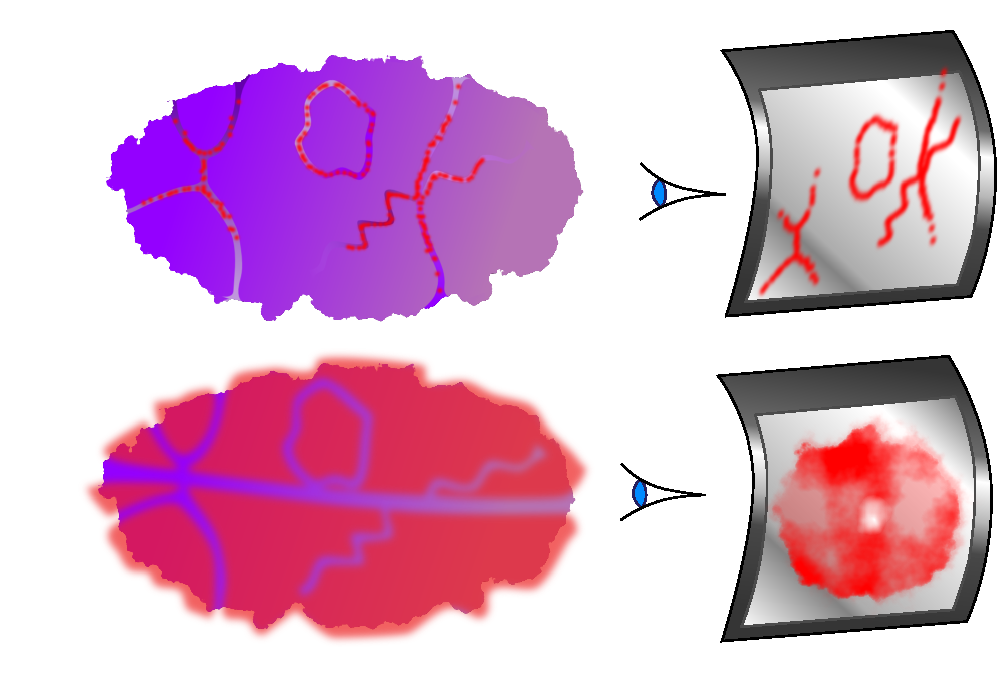
\includegraphics[width=0.6\textwidth]{figures/unsorted/side-on.pdf}
\caption{\label{fig:side-on}Imaging of the condensate itself, whether by fluorescence (bottom) or absorption imaging makes it difficult to resolve vortices unless they are viewed end-on. The vortex cores are usually smaller than the imaging wavelength, and are thus also difficult to resolve unless the cloud is allowed to expand. Imaging tracer particles instead (top) has the potential to resolve both problems.}\label{fig:side_on}
\end{center}
\end{figure}

This method has the potential to overcome several difficulties that imaging techniques face when used to image vortices. In ordinary absorption imaging, atoms are imaged via resonant absorption, and vortices---visible as density minima---generally can only be seen when the vortex line is parallel to the illumination. If not viewed end-on in this way, a vortex line represents only a minor decrease in column density and cannot be distinguished from the rest of the condensate (\figref{fig:side_on}). One solution to this problem is to slice the condensate into layers, and image them separately~\cite{anderson_watching_2001}.

The use of tracer particles that are only present within vortex cores allows vortex lines to be visible from any viewing angle.  Furthermore, since the atoms being imaged reside in the vortex cores themselves rather than the bulk of the condensate, this imaging can potentially be repeatedly or continuously performed without destroying the condensate. This may enable observation of the time evolution of Kelvin waves~\cite{bretin_quadrupole_2003}, vortex reconnections~\cite{leadbeater_sound_2001}, and vortex rings~\cite{anderson_watching_2001}.

This \emph{in-situ} imaging of vortex dynamics may allow more types of vortex motion to be imaged. Dynamics of \bec s are typically studied using a shot-by-shot method, in which repeated experiments with identical initial conditions are imaged destructively after being allowed to evolve for different amounts of time. Whilst this works for many types of dynamics, it fails for experiments that are sensitive to initial conditions and noise (quantum or otherwise), such as turbulent flow. This includes phenomena which cannot be created reliably in the same initial state, even though the evolution thereafter would be consistent from one experimental run to the next. One such phenomenon is the spontaneous generation of vortices after evaporative cooling~\cite{weiler_spontaneous_2008}.

\emph{In-situ} imaging of vortex motion has been achieved previously~\cite{freilich_real-time_2010}, by ejecting a fraction of the atoms from the condensate periodically and imaging them. This process is limited by depletion of the condensate, and was also used only to image vortices end-on. The fraction of the condensate being imaged was also allowed to freely expand before being imaged, since vortex cores are otherwise unable to be resolved by the wavelength of light used. Our proposed method would require neither free expansion or depletion of the condensate.

\section{Motivation: Turbulence}

It is commonly said that turbulence is one of the greatest unsolved problems of classical physics. But in what sense is it an unsolved problem? It is not a problem at all if your aim is reductionism---the Navier--Stokes equation adequately describes the evolution of a Newtonian fluid within its domain of validity, including rich turbulent phenomena such as turbulent boundary layers, Rayleigh--Bénard convection~\cite{ahlers_trend:_2009}, and energy cascades~\cite{foias_navier-stokes_2001}.
 
and the process of deriving it from the underlying motion of classical particles is well understood. It's turtles all the way down~\cite[p 1]{hawking_brief_1988}; what more could we ask for?

A demonstrative comparison might be with the field of statistical mechanics, as precisely the same statement can be made about the energy content and exchange between systems of particles. Statistical mechanics has revealed that despite the chaotic motion of individual particles in an ensemble, definite statements can still be made about the behaviour of the system as a whole, \emph{without having to consider the dynamics of the constituent components in detail}.

This is the kind of solution people have in mind when they speak of `solving' the problem of turbulence. Laws describing the average properties of a fluid without reference to its precise flow field would not simply be interesting because they describe turbulence as an emergent phenomenon, but would aid practical computations, which for many problems of interest are prohibitively computationally expensive. The flow of a turbulent fluid contains detail on such a  wide range of length scales that finite-element or finite-difference analyses of a system such as an aeroplane wing requires a very high resolution in order to be accurate. Following an estimate of computing power required to simulate a turbulent system down to its smallest length scales, Stanley Corrsin quipped~\cite{corrsin_turbulent_1961}:
\begin{quote}
The foregoing estimate  is enough to suggest the use of analog instead of digital  computation; in particular, how about an analog consisting of a tank of water?
\end{quote}
The reliance of the aerospace industry on wind tunnels and practical tests shows that there is some truth to the necessity of using nature as one's computer when it comes to turbulence. Whilst nature must always have the final say, it would be of great benefit to be able to compute expected results more cheaply before setting up a wind-tunnel experiment or constructing a prototype aircraft. Gaining predictive power through an improved ability to reason about turbulence would help escape to evolutionary model of testing and modifying prototypes of systems subject to turbulent flow.

But are we asking for too much? Perhaps the statistical properties of a turbulent fluid fundamentally cannot be decoupled from the finer details. There is reason to believe that this is not the case. There are several tantalising results that hint at universal properties that all turbulent flows share, and there is the simple empirical observation that the average flow of turbulent fluids at large scales is reproducible from one experimental run to the next~\cite[pp 13, 86]{davidson_turbulence:_2004}.

One of these universal results is Kolmogorov's theory of the statistics of small eddies~\cite{kolmogorov_local_1941, spalding_kolmogorovs_1991}. Another is the fact that the rate of energy dissipation via the action of viscosity at small scales is independent of the viscosity itself~\cite[p 77]{davidson_turbulence:_2004}. Then there is the Richardson energy cascade~\cite{richardson_weather_2007}, in which energy is continually transferred from larger scales to smaller scales. With dissipation at the smallest scales and energy injection at larger scales, this allows for the existence of `steady state' turbulence.

The above examples derive from ordinary, viscous fluids. Bose--Einstein condensates on the other hand are superfluids. There are several interesting aspects of superfluid turbulence that differ from classical turbulence. The defining difference is the absence of viscosity; another major difference is the quantisation of circulation. On length scales much larger than spacing between vortex lines, superfluid turbulence is expected to closely resemble classical turbulence~\cite{tsubota_energy_2009}. At smaller scales however the energy dissipation mechanism is different, instead involving the production of sound waves via vortex interactions~\cite{tsubota_energy_2009, vinen_how_2005}.

In certain 2\textsc{d} geometries, an \emph{inverse cascade}~\cite{onsager_statistical_1949, kraichnan_inertial_1967} is predicted to take place in superfluids, whereby energy moves not from large scales to small, but from small to large, clustering quantised vortices of the same circulation direction together. This phenomenon has been studied theoretically and numerically in the Monash Quantum Fluids group~\cite{simula_emergence_2014, groszek_vortex_2018} and recently experimentally observed in the Monash Dual-Species laboratory in experiments performed by Shaun Johnstone~\cite{johnstone_order_2018}, simultaneously with a group at the University of Queensland~\cite{gauthier_negative-temperature_2018}.

\subsection{Characterisation of turbulence as vortex dynamics}

The following definition of turbulence, taken from~\cite[p 53]{davidson_turbulence:_2004}, emphasises the role of vortices in turbulence in general:
\begin{quote}
Incompressible hydrodynamic turbulence is a spatially complex distribution of vorticity which advects itself in a chaotic manner in accordance with [the vorticity equation\footnote{The vorticity equation is a transformation of the Navier--Stokes equation for an incompressible fluid into a form that describes the vorticity field directly, rather than the velocity field.}]. The vorticity field is random in both space and time, and exhibits a wide and continuous distribution of length and time scales.
\end{quote}

When vorticity exists only in infinitesimally narrow lines, as it does in a superfluid, the vorticity equation mentioned in the above definition reduces to a Biot--Savart-type law which can be used to compute the motion of vortices without having to compute the entire flow field. This is why we are interested in the study of the dynamics of quantised vortices. Unlike in classical fluids, the vortices in superfluids have a definite position and size; there either is a vortex line within a given spatial region or there is not. This may make it simpler to describe the motion of vortices statistically.

So far experimental studies of superfluid turbulence have been primarily in the context of liquid helium~\cite{leggett_superfluidity_1999}. Bose--Einstein condensates offer a compelling alternative subject of study for superfluid turbulence. The high degree of control afforded over systems of cold atoms allows superfluid properties to be tweaked in several ways, such as modifying their density, temperature, trapping potential, interaction strength, or even the effective mass of fluid particles via the application of a periodic potential. This control creates a larger parameter space in which to study turbulence than that afforded by liquid helium.

Vortices are the skeletons of turbulence---to study turbulence via the behaviour of vortices, we need to track them.

\section{Overview of velocimetry scheme}

\begin{figure}
\begin{center}
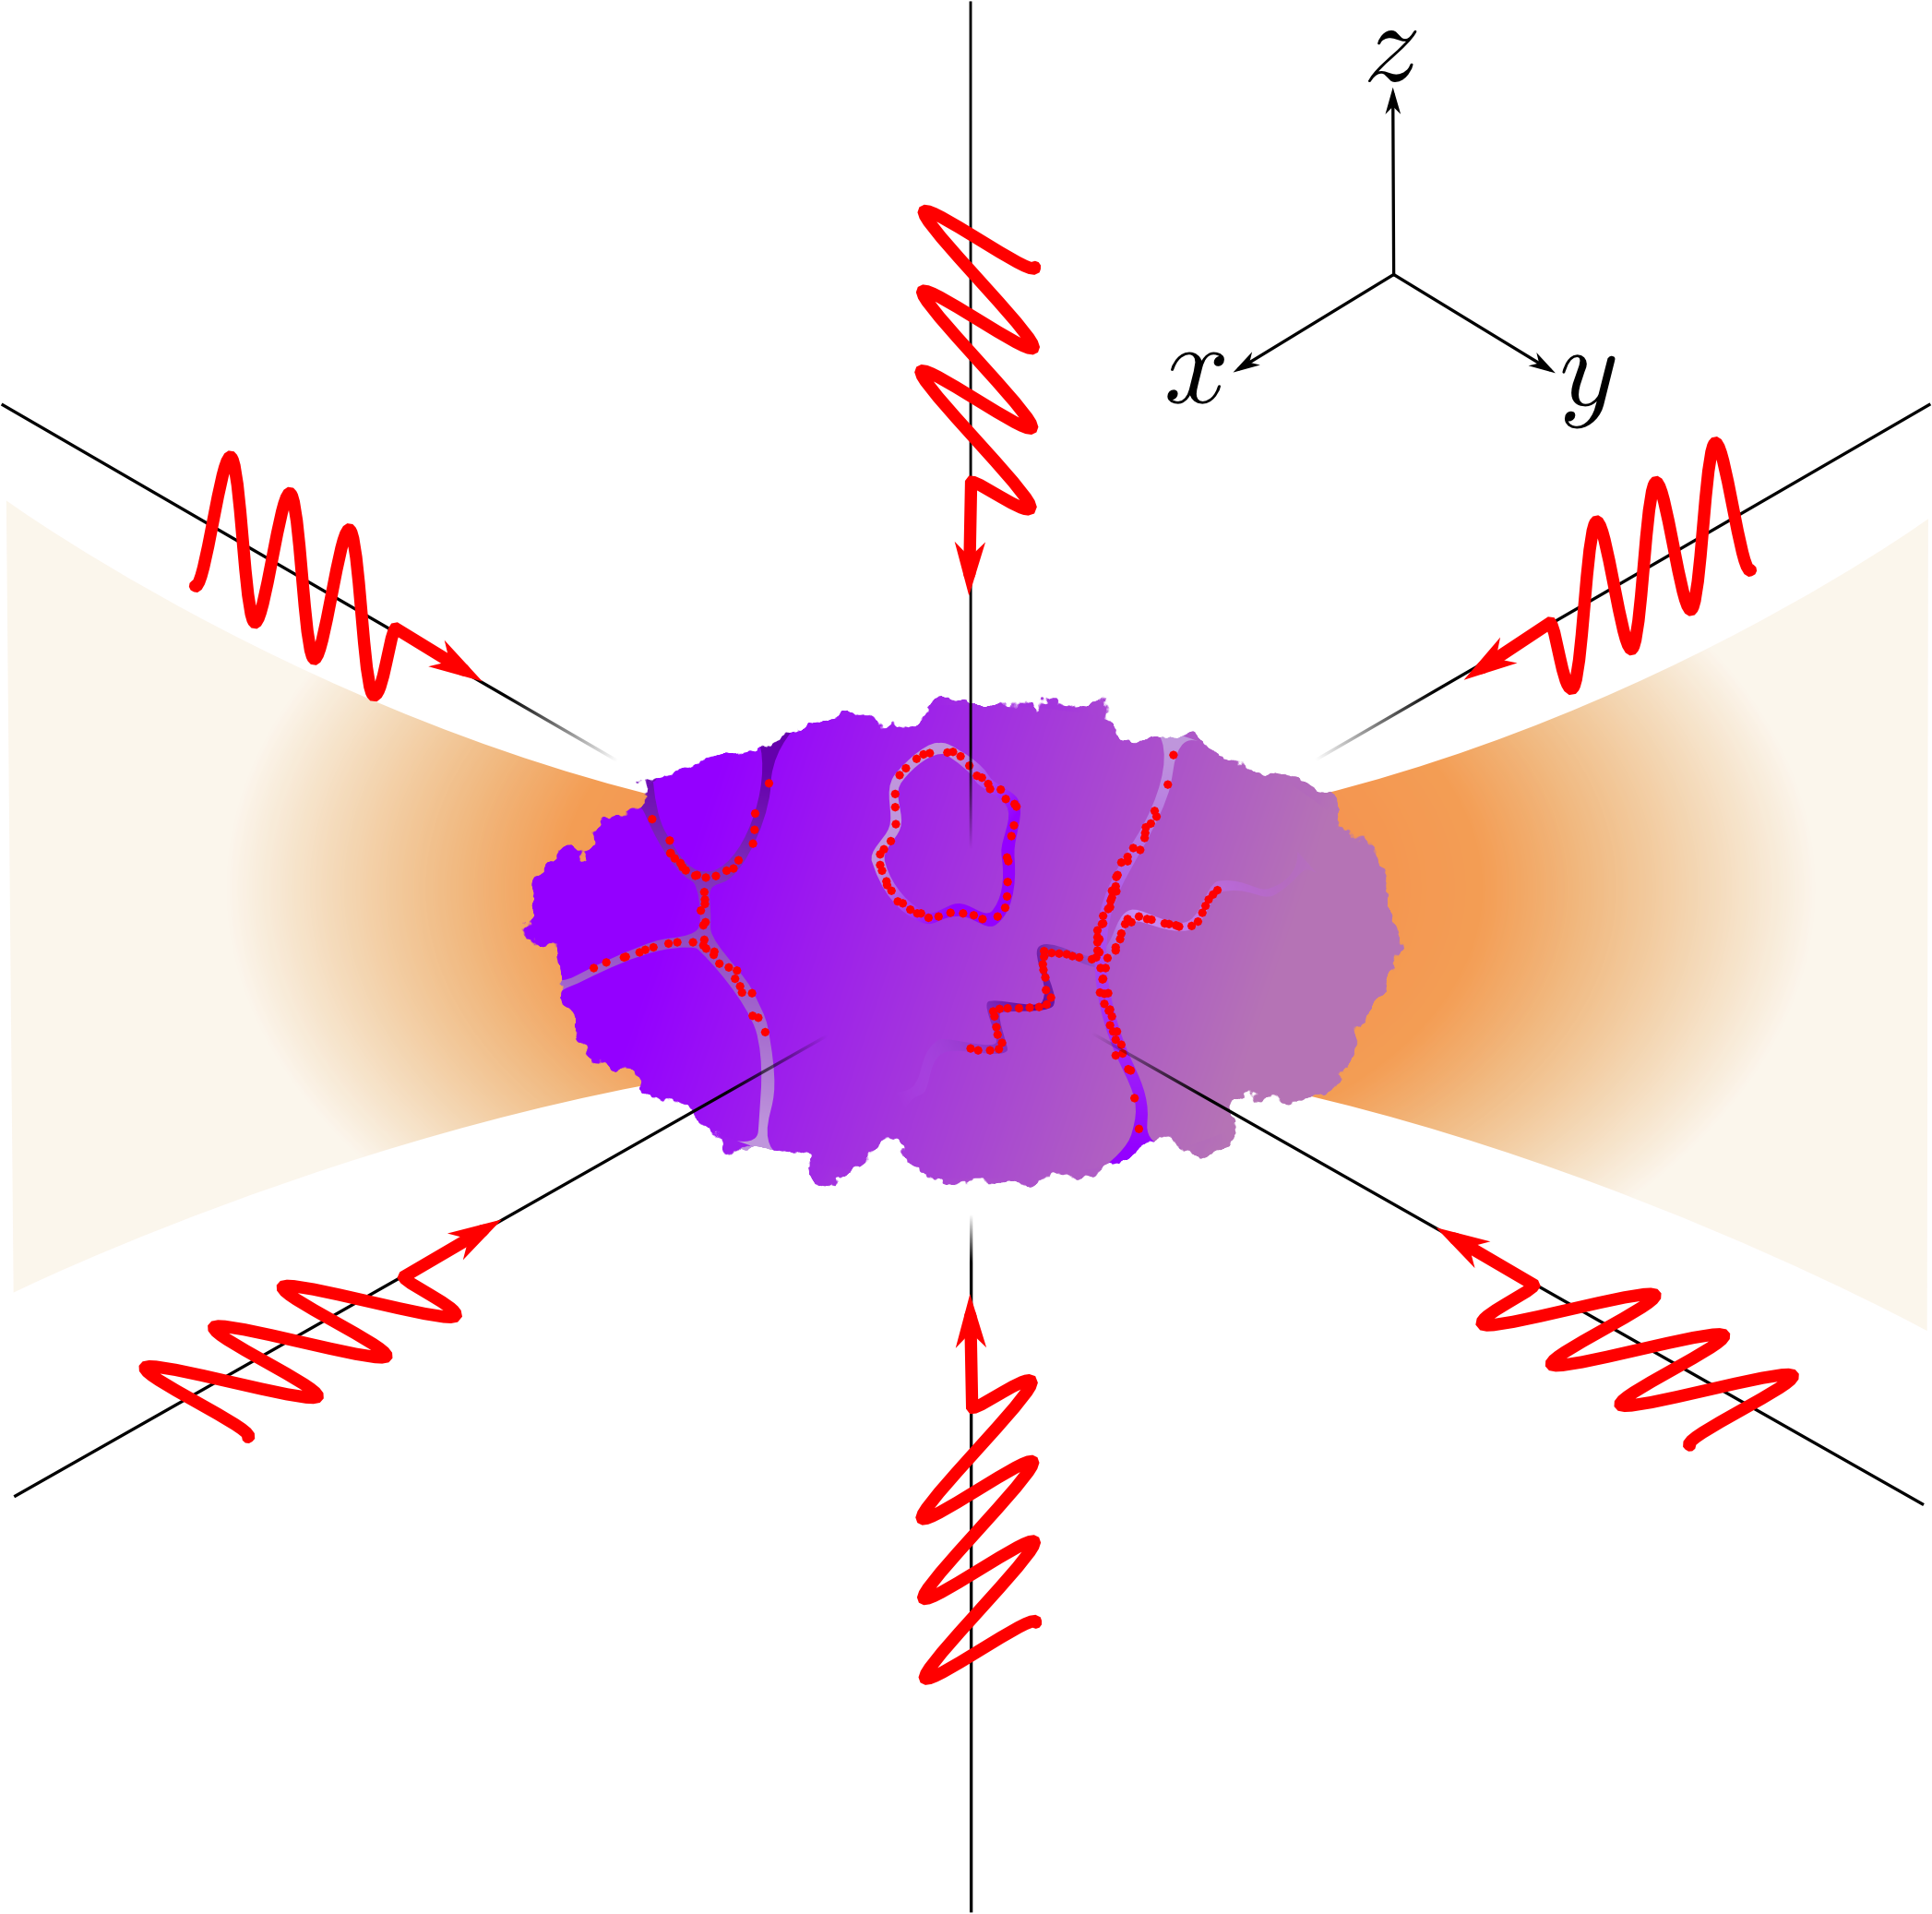
\includegraphics[width=0.6\textwidth]{figures/unsorted/setup.png}
\caption{\label{fig:setup}The simplest scheme for cooling and imaging the tracer particles with the same light is polarisation gradient cooling: six red-detuned beams (red), with each counter-propagating pair having opposite linear polarisations. Light scatters off the tracer atoms and cools them to sub-Doppler temperatures. If the cooling is sufficient, atoms move into the vortex cores where their energy is lower, if they aren't already there. Both the rubidium tracers and the potassium \bec\ are trapped with approximately the same trapping potential by a strong, far off-resonant laser (orange), via the dipole force. Magnetic trapping cannot be used, as polarisation gradient cooling does not work in the presence of a magnetic field.}
\end{center}
\end{figure}

As mentioned, the core idea of our proposed imaging method is to use tracer particles to track vortex cores in a \bec. In this chapter I consider $^{87}$Rb atoms as tracer particles in a \textsc{bec} made of $^{41}$K. This choice is due to the strong interspecies repulsion between these atomic species, which gives rise to the trapping of atoms in the vortex cores. In the limit of low densities and temperatures, such that three body collisions are suppressed and $s$-wave scattering dominates the interspecies interactions~\cite[p 120]{leggett_quantum_2006}, the rubidium tracer atoms experience a potential due to the potassium:

\begin{equation}
V(\vec{r}) = \frac{2\pi\hbar^2 a_s}{m_r}\rho_\up{K}(\vec{r}),
\end{equation}
where $\rho_\up{K}(\vec{r})$ is the spatially varying atom density of the potassium condensate, $a_s$ is the interspecies $s$-wave scattering length, and
$m_r = \frac{m_\up{K}m_\up{Rb}}{m_\up{K} + m_\up{Rb}}$ is the reduced mass of the scattering pair. Vortex cores thus create potential wells for other atoms, since they are regions of low condensate density in a background of higher density.

The scheme is shown in Figure~\ref{fig:setup}. Cold rubidium atoms are introduced (possibly via magnetic transport from a cold--but not necessarily condensed---source) to a potassium condensate, after which both species are optically trapped at the focus of a high power $1064$nm laser, using the dipole force. Various methods may be used to create vortices in the condensate. These include bluff-body flow, where a repulsive potential is dragged through the condensate, or inducing a turbulent state by applying off-resonant laser speckle. The rubidium atoms are then expected to become trapped in the low density vortex cores.

The tracer atoms are imaged with resonant or near-resonant laser light, depending on the exact scheme employed. The scattering of imaging photons heats the tracer atoms, which, if sufficient to cause them to escape the vortex cores, presents a problem for acquiring images of vortex motion. In Section~\ref{sec:sympathetic} I present the results of simulating tracer atoms imaged with resonant light. This light does not provide any cooling, instead the simulation includes the cooling effect of the condensate itself. These results show that sympathetic cooling of the tracer atoms by the condensate may be sufficient to retain tracer atoms in vortices whilst scattering imaging light.

The simplest scheme which attempts to laser-cool the rubidium atoms is ordinary polarisation gradient cooling, in which the same light is used for imaging and cooling the atoms (Figure~\ref{fig:setup}). This was considered in my Honours thesis~\cite{billington_particle_2010}, the results of which I summarise in the next section. This method precludes the use of a magnetic trap or large bias field, since either would destroy the cooling effect.

The vortex potentials may be made deeper through the use of a Feshbach resonance (Section~\ref{sec:feshbach}), which increases the interspecies scattering length. However, since this requires a magnetic field, it precludes the use of ordinary polarisation gradient cooling. In section (see Section~\ref{sec:laser_cooling_simulations}) I present an alternative polarisation gradient cooling scheme designed work in the presence of a magnetic field of the strength required for the Feshbach resonance of interest.

Effective imaging of vortex motion would require approximately $10^5$ photons per second to scatter off each rubidium atom without it escaping its vortex core trap, and without causing so much heating as to destroy the condensate on a reasonable experimental timescale. A high resolution, low aberration lens (numerical aperture $\approx 0.5$) would also be required to focus the scattered light onto a fast capture, high quantum efficiency camera to produce images of vortex motion.

\section{Relation to previous work}

This scheme was first investigated in my Honours project~\cite{billington_particle_2010}. In that work I investigated the ability of vortex potentials to trap atoms, including consideration of the depth of such traps when measured in units of the photon recoil energy. Considering the depth in these units was a first attempt to estimate how easily atoms may escape vortex potentials in the presence of imaging light. Figure~\ref{fig:levels1e14} and Figure~\ref{fig:levels1e15} show bound states of typical vortex potentials at different condensate densities.

\begin{figure}
\centering
\noindent\makebox[\textwidth]{
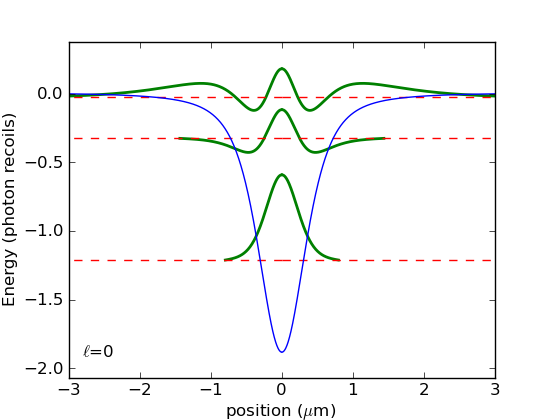
\includegraphics[width=0.5\columnwidth]{figures/velocimetry/levels1e14_l=00.png}
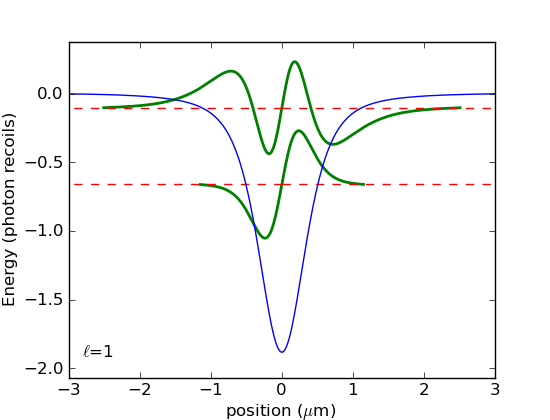
\includegraphics[width=0.5\columnwidth]{figures/velocimetry/levels1e14_l=01.png}}
\noindent\makebox[\textwidth]{
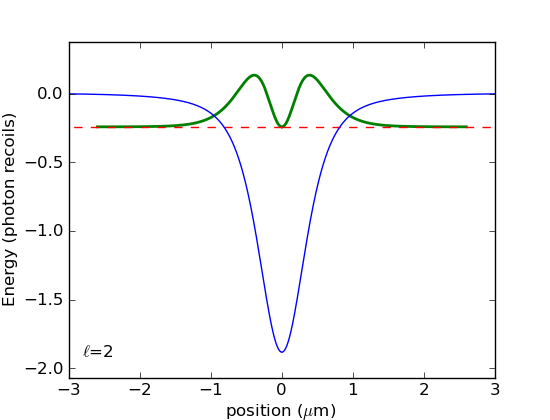
\includegraphics[width=0.5\columnwidth]{figures/velocimetry/levels1e14_l=02.png}
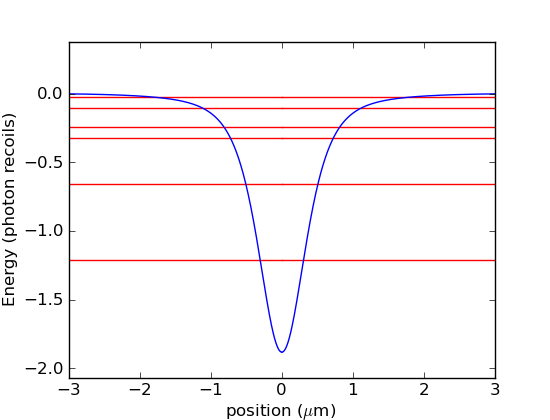
\includegraphics[width=0.5\columnwidth]{figures/velocimetry/levels1e14.png}}
\caption{Energy eigenstates of a rubidium atom in a potassium vortex core, for a potassium \textsc{bec} with background density $\approx 10^{14}\unit{cm}^{-3}$. There are a number of bound states spanning three orbital quantum numbers. Plots of the bound states are of a cross section through the centre of a vortex core, and the lower right plot shows just the energy levels (for all orbital quantum numbers $\ell$). Figure reproduced from~\cite{billington_particle_2010}.}%
\label{fig:levels1e14}%
\end{figure}

\begin{figure}
\centering
\noindent\makebox[\textwidth]{
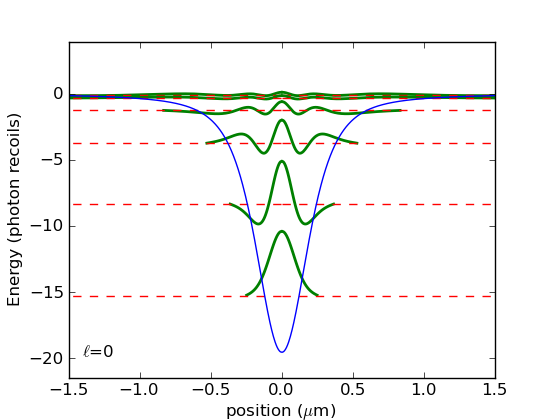
\includegraphics[width=0.5\columnwidth]{figures/velocimetry/levels1e15_l=00.png}
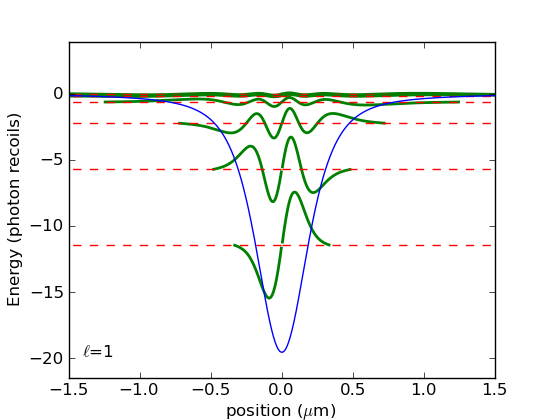
\includegraphics[width=0.5\columnwidth]{figures/velocimetry/levels1e15_l=01.png}}
\noindent\makebox[\textwidth]{
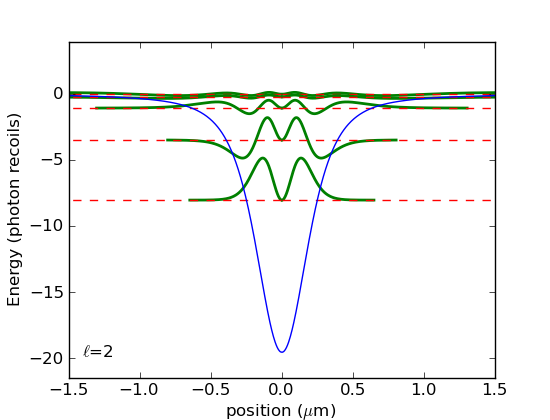
\includegraphics[width=0.5\columnwidth]{figures/velocimetry/levels1e15_l=02.png}
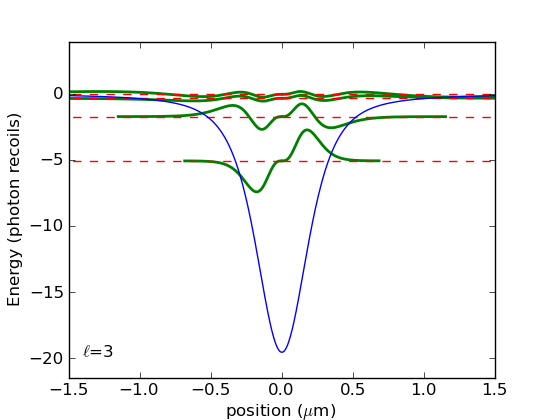
\includegraphics[width=0.5\columnwidth]{figures/velocimetry/levels1e15_l=03.png}}
\noindent\makebox[\textwidth]{
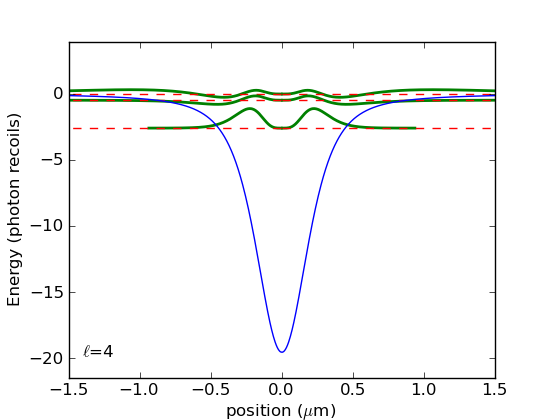
\includegraphics[width=0.5\columnwidth]{figures/velocimetry/levels1e15_l=04.png}
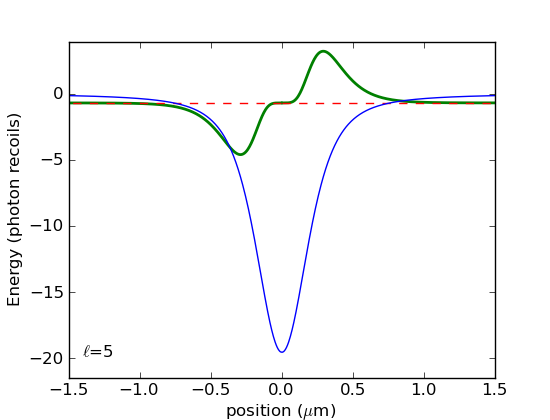
\includegraphics[width=0.5\columnwidth]{figures/velocimetry/levels1e15_l=05}}
\noindent\makebox[\textwidth]{
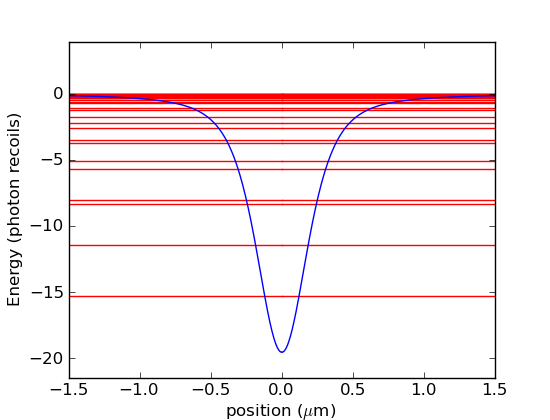
\includegraphics[width=0.5\columnwidth]{figures/velocimetry/levels1e15.png}}
\caption{As in Figure~\ref{fig:levels1e14}, but for a potassium \textsc{bec} with background density ${\approx 10^{15}\unit{cm}^{-3}}$. There are bound states over six different orbital quantum numbers. This vortex potential is much deeper than that in Figure~\ref{fig:levels1e14}, showing the effect of condensate density on the depth of the vortex potentials . Figure reproduced from~\cite{billington_particle_2010}.}%
\label{fig:levels1e15}%
\end{figure}

To minimise the recoil energy, rubidium is a better choice for tracer particle than potassium due to its larger mass, enabling a rubidium atom to scatter more photons before escaping a vortex potential compared to a potassium atom. Vortex potentials are not very deep when measured in recoil energies, and their depth depends strongly on the density of the \textsc{bec}. At typical condensate densities of $10^{14}\unit{cm}^{-3}$, the vortex potentials are expected to only be 1--2 recoil energies deep, making it unlikely that atoms could scatter many photons whilst remaining trapped in them. At larger densities of $10^{15}\unit{cm}^{-3}$, the vortex potentials are closer to $20$ recoil energies deep, making imaging of trapped tracer atoms more plausible.

The main simulation result of my Honours project considered a potassium condensate with a peak density of $10^{15}\unit{cm}^{-3}$ and rubidium tracer atoms being cooled using standard polarisation-gradient cooling with parameters chosen to ensure each atom scattered on the order of $10^5$ photons per second. The result was that initially randomly distributed rubidium atoms were able to become---and remain---trapped in the vortex cores whilst being cooled (Figure~\ref{fig:hybrid}).

\begin{figure}
\centering
\noindent\makebox[\textwidth]{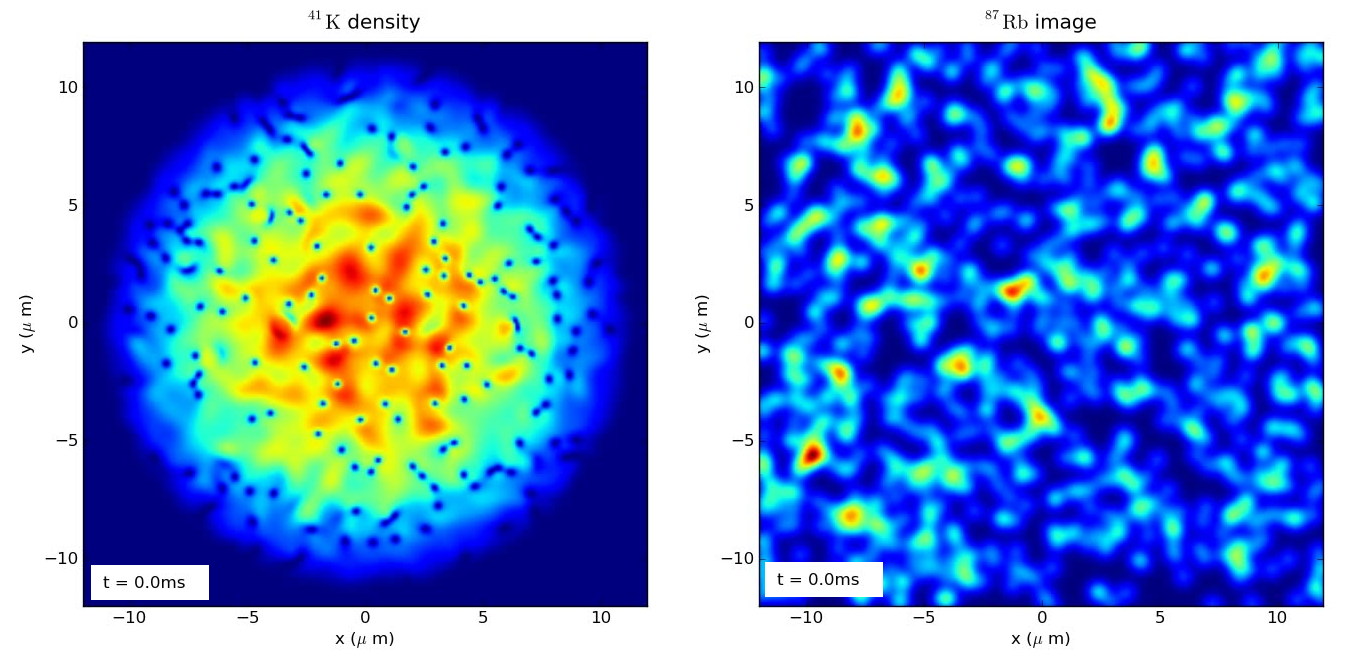
\includegraphics[width=1.0\columnwidth]{figures/velocimetry/hybrid1.png}}
\noindent\makebox[\textwidth]{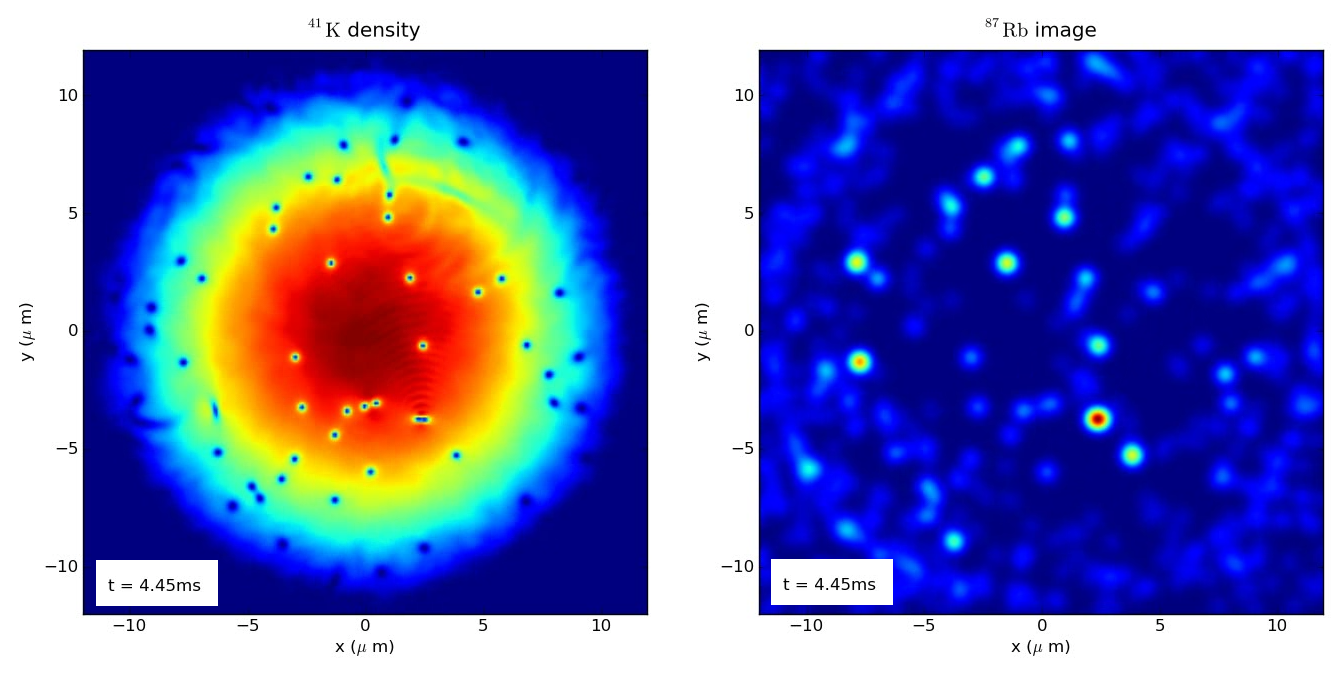
\includegraphics[width=1.0\columnwidth]{figures/velocimetry/hybrid2.png}}
\noindent\makebox[\textwidth]{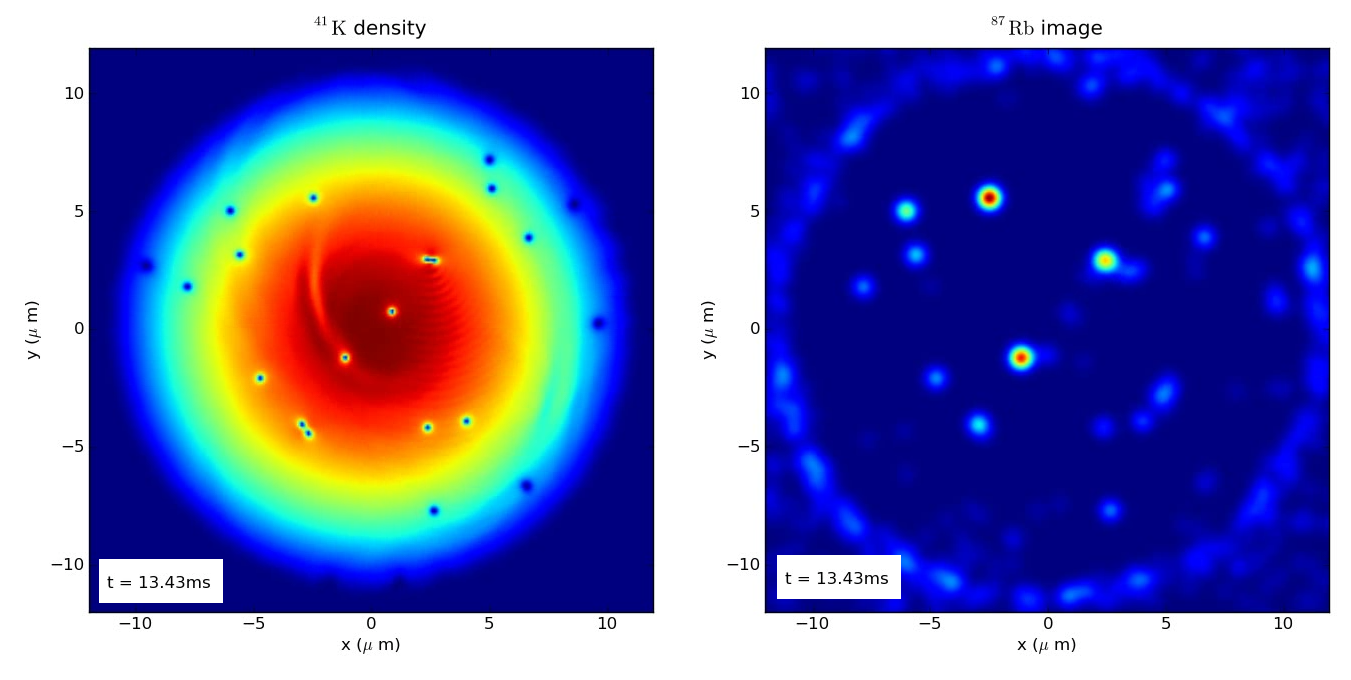
\includegraphics[width=1.0\columnwidth]{figures/velocimetry/hybrid3.png}}
\caption{The result from~\cite{billington_particle_2010} of a two-dimensional hybrid quantum-classical simulation for $1000$ classically modelled rubidium atoms (right, depicted as fluorescence assuming diffraction through an $\mathrm{NA}=0.5$ imaging system) and a turbulent potassium \textsc{bec} (left) of peak density $\approx 10^{15}\unit{cm}^{-3}$. The rubidium atoms are subject to a classical approximation of the force due to polarisation gradient cooling as described in~\cite{billington_particle_2010}. Most rubidium atoms eventually either become bound to a vortex core or leave the condensate. Figure reproduced from~\cite{billington_particle_2010}.}%
\label{fig:hybrid}%
\end{figure}

However, the density assumed in this simulation was rather high for a real experiment. Three-body losses tend to limit the lifetime of condensates at such a high density, and so the work in this chapter investigates ways to make particle velocimetry work in a less dense condensate through the use of a Feshbach resonance.

In Section~\ref{sec:sympathetic} I consider a similar configuration, but with a more reasonable \textsc{bec} density combined with an enhancement of the interspecies repulsion due to the Feshbach resonance. I investigate whether sympathetic cooling of the tracer atoms by the condensate may be enough to keep them trapped in the presence of imaging light. Then, in Section~\ref{sec:laser_cooling_simulations} I present simulation results of a new laser cooling scheme designed to work at the magnetic field strength required for the Feshbach resonance.

\section{Sympathetic cooling}\label{sec:sympathetic}

The simulation performed in my Honours thesis considered only polarisation gradient cooling counteracting the heating effect of the imaging light. In reality, collisions between tracer atoms and atoms in the condensate would also contribute to cooling of the rubidium. This sympathetic cooling of the tracer atoms---which would also lead to heating of the condensate---was disregarded in my Honours results. 

Depending on the strength, sympathetic cooling may be sufficient to retain tracer atoms in vortex cores in the absence of an additional cooling mechanism. If laser cooling is not necessary to trap tracer atoms in vortices, then the Feshbach resonance may be used to enhance the interspecies scattering length, further enhancing the ability of the vortices to trap tracer atoms. In this section I consider a similar simulation to that in my Honours thesis, except with no laser cooling simulated, and with a model of sympathetic cooling taken into account, in order to examine this possibility.

\subsection{Model}

In this section I model sympathetic cooling as elastic two-body scattering between the rubidium tracer atoms and the potassium atoms in the condensate. The model is two-dimensional, appropriate for a pancake-shaped condensate. As with the simulation in my Honours thesis, I model the \textsc{bec} with the damped Gross--Pitaevskii equation:
\begin{align}
\ii\hbar\pdv{t} \Psi_\up{K}(\vec r, t) = (1-\ii\gamma)\left[-\frac{\hbar^2}{2m_\up{K}}\nabla^2 + V(\vec{\vec r}) + g_\up{K}\abs{\Psi_\up{K}(\vec r, t)}^2\right]\Psi_\up{K}(\vec r, t),
\end{align}
with damping constant $\gamma=0.01$ and all other symbols are as defined in Section~\ref{sec:mean_field_theory}, with the added subscripts $\up{K}$ indicating quantities specific to $^{41}\up{K}$. The $^{41}$K $s$-wave scattering length is $a_\up{K}=121 a_0$~\cite{cote_potassium_1998}, where $a_0$ is the Bohr radius. The damped \textsc{gpe}~\cite{tsubota_vortex_2002, madarassy_vortex_2008} is a phenomenological modification of the standard \textsc{gpe} that includes dissipation to gradually remove higher energy excitations from the condensate wavefunction, approximating behaviour at finite-temperature. The condensate wavefunction is normalised at each timestep to compensate for the decay this model otherwise would cause. The potential $V(\vec r)$ is a harmonic potential $ V(\vec r) = \frac12m_\up{K}\omega_\up{K}^2 r^2$.

The rubidium tracer atoms are modelled classically, evolving under the potential due to interspecies repulsion, as well as the external potential\footnote{For simplicity I assume that both species are subject to the same external potential. Writing the potential as a harmonic trap for rubidium such that $V(\vec r) = \frac12m_\up{K}\omega_\up{K}^2 r^2 = \frac12m_\up{Rb}\omega_\up{Rb}^2 r^2$ gives $\omega_\up{Rb} \approx 0.7\omega_\up{K}$.} $V(\vec r)$, resulting in the equation of motion:
\begin{align}\label{eq:classical_motion_tracers}
\dv[2]{t} \vec r = -\frac1{m_\up{Rb}}\nabla\left({g_{\textrm{Rb--K}}} \abs{\Psi_\up{K}(\vec r, t)}^2 + V(\vec r)\right),
\end{align}
where $g_{\textrm{Rb--K}}$ is the $^{87}$Rb--$^{41}$K non-linear interaction constant $g_{\textrm{Rb--K}} = \frac{2\pi\hbar^2 a_{\textrm{Rb--K}}}{m_\up{r}}$,
with $m_\up{r}$ the reduced mass of the $^{87}$Rb--$^{41}$K scattering pair and 
$a_{\textrm{Rb--K}}$ the $s$-wave interspecies scattering length. $a_{\textrm{Rb--K}}$ is equal to $640 a_0$ at zero magnetic field~\cite{thalhammer_double_2008}, and assumed in this section to be enhanced by a factor of five by means of the $34\unit{G}$ Feshbach resonance (see Section~\ref{sec:feshbach} and \figref{fig:feshKRb}). Since the Gross--Pitaevskii equation is solved on a grid whereas the classical motion of the atoms is modelled using continuous position variables, the condensate density is numerically differentiated and the results interpolated to the positions of the tracer atoms using cubic splines in order to evaluate~\eqref{eq:classical_motion_tracers} for each tracer atom.


The motion of the tracer atoms is punctuated by momentum jumps due to both the scattering of imaging photons and two-body collisions with the condensate. Photon scattering events are modelled as instantaneous momentum jumps of magnitude $hc/\lambda$ where $\lambda=780\unit{nm}$ is the wavelength of the imaging light. A random direction in \textsc{3d} space is chosen and a momentum jump in this direction with the given magnitude is projected into the \textsc{2d} plane of the simulation before being applied to the atom. These jumps occur at random times at an average rate given by the target photon scattering rate of $10^5$ photons per second. Neglecting the exact details of the imaging light used, I assume repumping is included such that the atom spends nearly all of its time in the $\ket{1, 1}$ ground state---necessary for the scattering length enhancement---and that the target scattering rate includes scattering from all lasers, repump or otherwise.

Collisions with the condensate are modelled as elastic collisions between a rubidium atom with the given classical velocity, and a potassium atom of velocity equal to the superfluid velocity $\vec v_\up{K}$ of the condensate (discussed in Section~\ref{sec:mean_field_theory}) at the location of the tracer atom, given by
\begin{align}
\vec v_\up{K}(\vec r, t) = \frac \hbar {m_\up{K}} \nabla \phi_\up{K}(\vec r, t),
\end{align}
where $\phi_\up{K}(\vec r, t)$ is the complex phase of the potassium condensate wavefunction. The $s$-wave scattering length $a$ is defined as~\cite[p 589, eq.~12.101]{bransden_physics_2003}
\begin{align}
a = -\lim_{k_\up{rel}\rightarrow 0} \frac{\tan\left(\delta_0(k_\up{rel})\right)}{k_\up{rel}},
\end{align}
where $k_\up{rel}=m_\up{r}v_\up{rel}/\hbar$ is the relative wavenumber of the colliding pair of atoms with reduced mass $m_\up{r}$ and relative velocity $v_\up{rel}$, and $\delta_0(k)$ the collisional phase shift. Assuming small $k_\up{rel}$ and substituting this into the $s$-wave elastic scattering cross section~\cite[p 584, eq.~12.66]{bransden_physics_2003} 
\begin{align}
\sigma = \frac{4\pi}{k_\up{rel}^2}\sin^2\left(\delta_0(k_\up{rel})\right)
\end{align}
gives a low-velocity approximation to the scattering cross section for elastic collisions between the rubidium and potassium atoms:
\begin{align}\label{eq:sigma_scattering}
\sigma_{\textrm{Rb--K}} \approx 4\pi\frac{a_{\textrm{Rb--K}}^2}{1 + k_\up{rel}^2a_{\textrm{Rb--K}}^2}.
\end{align}
For rubidium atoms at $5\unit{\upmu K}$, $k_\up{rel}a_{\textrm{Rb--K}} < 0.1$, such that the zero-velocity scattering cross section $\sigma = 4\pi a^2$ would be accurate enough; nonetheless~\eqref{eq:sigma_scattering} is the expression used in this section.\footnote{For modestly larger Feshbach enhancements of the scattering length, the zero-velocity cross section would not be accurate and the velocity dependence of the scattering cross section would become important.} From the scattering cross section we obtain the mean free path of a rubidium tracer particle within the potassium \textsc{bec}:
\begin{align}
\ell(\vec r, t) = \left(\sigma_{\textrm{Rb--K}}\abs{\Psi_\up{K}(\vec r, t)}^2\right)^{-1},
\end{align}
yielding the probability of a collision occurring in an infinitesimal time interval $\dd t$:
\begin{align}\label{eq:P_collision}
P_\up{collision}(\vec r; t, t+\dd t) = v_\up{rel}(\vec r, t)\sigma_{\textrm{Rb--K}}\abs{\Psi_\up{K}(\vec r, t)}^2\dd t,
\end{align}
where $v_\up{rel} = \abs{\vec v_\up{K}(\vec r, t) - \vec v}$ for a specific rubidium atom at position $\vec r$ and with velocity $\vec v$.

At each timestep, a random number between zero and one is generated for each atom, and if less than~\eqref{eq:P_collision}, a collision is taken to have occurred.\footnote{During thesis writing, an error was discovered in the code that produced the results in this section, in which the computed collision probability~\eqref{eq:P_collision} was too small by a factor of $\sqrt{2}$. As such, the results shown in the next subsection underestimate the sympathetic cooling effect slightly. I do not expect this error to change any of my conclusions.} In the case of a collision, the \textsc{2d} elastic scattering problem is solved and the rubidium atom's velocity instantaneously replaced with its post-collision value. The potassium condensate wavefunction is not modified---the sympathetic heating resulting from these collisions is ignored, which is a limitation of these results. For an ideal Bose gas of $10^6$ potassium atoms at $T = T_\up{c}/2$, a heating rate of $10^5$ rubidium recoil energies per second from each of $10^3$ rubidium represents a rate of temperature increase of $25\unit{nK\,ms}^{-1}$. This suggests that relying on sympathetic cooling alone may not allow for imaging of vortex motion for more than a few milliseconds (after which the condensate temperature will exceed the critical temperature), and that further cooling such as that presented in Section~\ref{sec:laser_cooling_simulations} may be necessary.

\subsection{Results}

I simulated the equations described in the previous section in two dimensions, with the \textsc{gpe} solved on a $256\times256$ grid using fourth-order Runge--Kutta (Section~\ref{sec:rk4}) with $\upDelta t = 500\unit{ns}$ using fast Fourier transforms to evaluate the kinetic energy term (Section~\ref{sec:fourier_pseudospectral}), and the tracer atom Newtonian equations of motion propagated also using fourth-order Runge--Kutta with the same timestep, for $10^3$ tracer atoms. The first derivatives of the condensate wavefunction required to compute its phase gradient were evaluated using second-order finite differences, which I observed to be less susceptible to Gibbs' phenomenon in the vicinity of vortex cores, which---when using Fourier transforms---would produce a velocity field with unphysical radial motion close to a vortex core.\footnote{Interestingly, second derivatives---as required for the kinetic energy term of the \textsc{gpe}---do not appear to suffer from this problem at similar grid resolutions.}

I repeated the simulation with two harmonic trapping frequencies in order to model two condensate densities. In the higher density simulations I used $\omega_\up{K}=2\pi\times 130\unit{Hz}$ and simulated a spatial region of $40\unit{\upmu m}\times40\unit{\upmu m}$. In the lower density simulations I used $\omega_\up{K}=2\pi\times 65\unit{Hz}$ and increased the size of the simulated region to $57\unit{\upmu m}\times57\unit{\upmu m}$.

I computed the initial conditions for the condensate wavefunction using the imaginary time evolution method (Section~\ref{sec:ITEM}) subject to a fixed \textsc{2d} normalisation constant leading to a peak density of $5.1\times 10^{14}\unit{cm}^{-3}$ for the higher density simulation and $2.5\times 10^{14}\unit{cm}^{-3}$ for the lower density simulation. Once the ground state condensate wavefunction was found, I then constructed a turbulent state by imposing a phase pattern on the condensate on a $16\times16$ grid, with the phase in each region chosen randomly from the interval $(-\pi, \pi)$. I then applied the imaginary time evolution algorithm once more for $600\unit{\upmu s}$ to produce a physically realistic condensate wavefunction containing a number of vortices randomly distributed.

The initial positions of the tracer atoms were uniformly distributed over the entire spatial region, and velocities drawn from a Maxwell--Boltzmann distribution at $5\unit{\upmu K}$.

After producing the initial conditions, I then evolved the system in time for $32\unit{ms}$ with sympathetic cooling being modelled, but `dark'---with zero photon scattering. The results of this are shown in Figure~\ref{fig:evolution_high_density} for the higher density case and Figure~\ref{fig:evolution_low_density} for the lower density. During this evolution many of the tracer atoms either moved into vortex cores or left the condensate (those that left mostly formed a ring at the Thomas--Fermi radius where the external potential and interspecies potential resulted in a potential minimum), showing that sympathetic cooling under the assumptions of this model is sufficient to cause randomly-distributed tracer atoms to become bound to vortex cores. During this evolution the vortices moved about the condensate, and due to the inclusion of damping, reduced in number over time as they left the condensate, or annihilated with each other.

I then continued this simulation, but with the inclusion of photon scattering as described in the previous section. For both the lower and higher density simulations, I used two timepoints in the dark simulations as initial conditions: $16\unit{ms}$ and $32\unit{ms}$. This was in order to examine whether the decay in vortex number over time improved the visibility of vortices in the resulting images, since there are fewer vortices at later times. Imaging was simulated for $10\unit{ms}$, and the location of each photon emission recorded in order to accumulate a simulated image of the tracer particle locations over time. From this idealised image---which does not include sub-unity collection efficiency or diffraction---I derived a more realistic image assuming $4.2 \%$ collection efficiency, and diffraction modelled as a displacement in the location of each detected photon by a random distance drawn from a Gaussian distribution with a standard deviation of $0.32\unit{\upmu m}$. This collection efficiency and spot size are appropriate for a $\up{NA}=0.5$ imaging system, assuming unit quantum efficiency of the camera sensor and a Gaussian approximation to the diffraction spot shape. No effort was made to include photons based on their emission direction.

The results are encouraging---vortex motion is clearly visible in the idealised images, and still quite visible in the more realistic images taking into account imperfect imaging. Contrary to expectations, at lower densities vortex traces are slightly more visible in the simulated images due to the slower motion of the vortices. Even though vortex potentials are only a few photon recoil energies in depth at the lower density, the simulated sympathetic cooling is effective at keeping the tracer atoms trapped within vortex cores. The modelled interaction between the tracer particles and the condensate causes the tracer particles to follow the local superfluid flow, including orbiting vortex cores prior to falling into them, and moving in circles within vortex cores once trapped.


\afterpage{
    \newgeometry{left=1in,bottom=1in,right=1in,top=1.5in}
    \begin{sidewaysfigure}[th]
    \centerfloat
    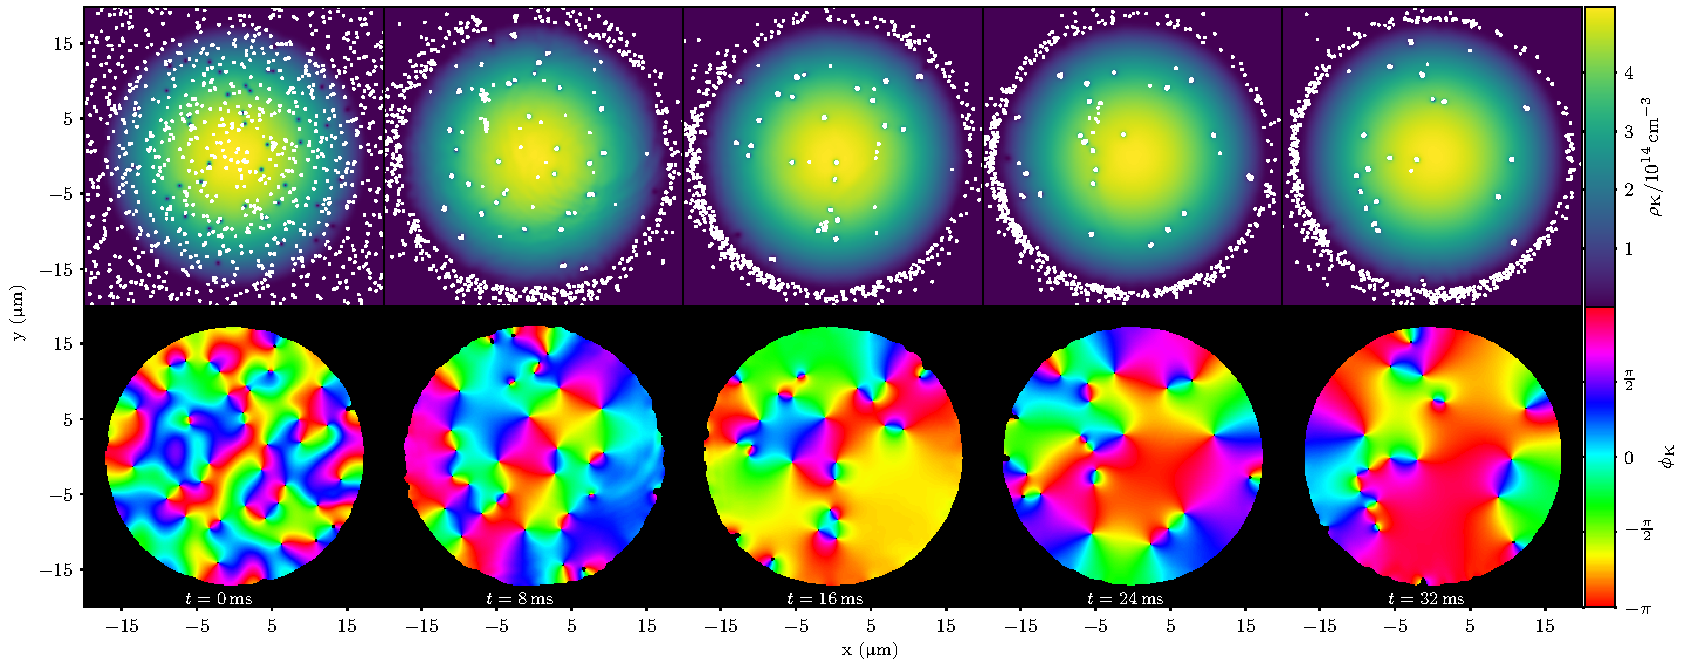
\includegraphics[width=1.05\textwidth]{figures/velocimetry/evolution_high_density.pdf}
    \caption{Higher density simulation of the evolution of the potassium condensate and $10^3$ rubidium tracer particles interacting via sympathetic cooling, beginning from a turbulent condensate with randomly distributed tracer particles. Top row: condensate density (false colour) and tracer particle positions (white dots). Bottom row: condensate phase showing the location of vortices as points about which the phase winds by $2\pi$. The initially randomly distributed tracer particles either leave the condensate or become trapped in vortex cores. When vortices annihilate, any tracer particles previously held remain in the condensate, this is an ongoing source of tracer particles in the bulk of the condensate that are not bound to vortex cores. Although not visible in these plots, in a video of these results the tracer particles can be seen to move in circles within vortex cores in the same direction of the superfluid flow.}
    \label{fig:evolution_high_density}
    \end{sidewaysfigure}
    \restoregeometry
}


\afterpage{
\newgeometry{left=1in,bottom=1.5in,right=1in,top=1.5in}
\begin{figure}
\centerfloat
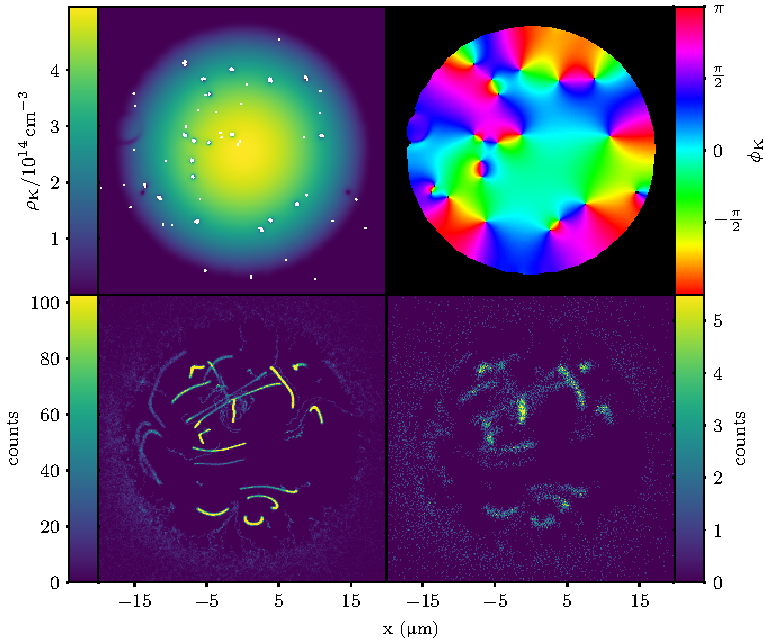
\includegraphics{figures/velocimetry/imaging_high_densitynormal_start.pdf}
\caption{Final state of the higher density simulation of imaging of tracer particles in the \textsc{bec} for $10\unit{ms}$ starting from the state of the `dark' simulation at $16\unit{ms}$ (i.e.~the central pair of Figure~\ref{fig:evolution_high_density}). Top left: The condensate density (false colour) and tracer particle positions (white dots). Tracer atoms that in the dark simulation formed a ring at the Thomas--Fermi radius are highly excited in the harmonic trap due to photon scattering, and leave the frame. Top right: condensate phase, showing the position of vortices as points about which phase winds by $2\pi$. Bottom left: idealised image of tracer particle photon emissions over the imaging period. Photon emission locations are binned into a $256\times256$ grid. Complex vortex motion is clearly visible. Bottom right: modelled image taking into account non-unity collection efficiency and diffraction. Photon counts are low, but more than half the vortices are usefully tracked.}\label{fig:imaging_high_densitynormal_start}
\end{figure}
\restoregeometry
}


\afterpage{
\newgeometry{left=1in,bottom=1.5in,right=1in,top=1.5in}
\begin{figure}
\centerfloat
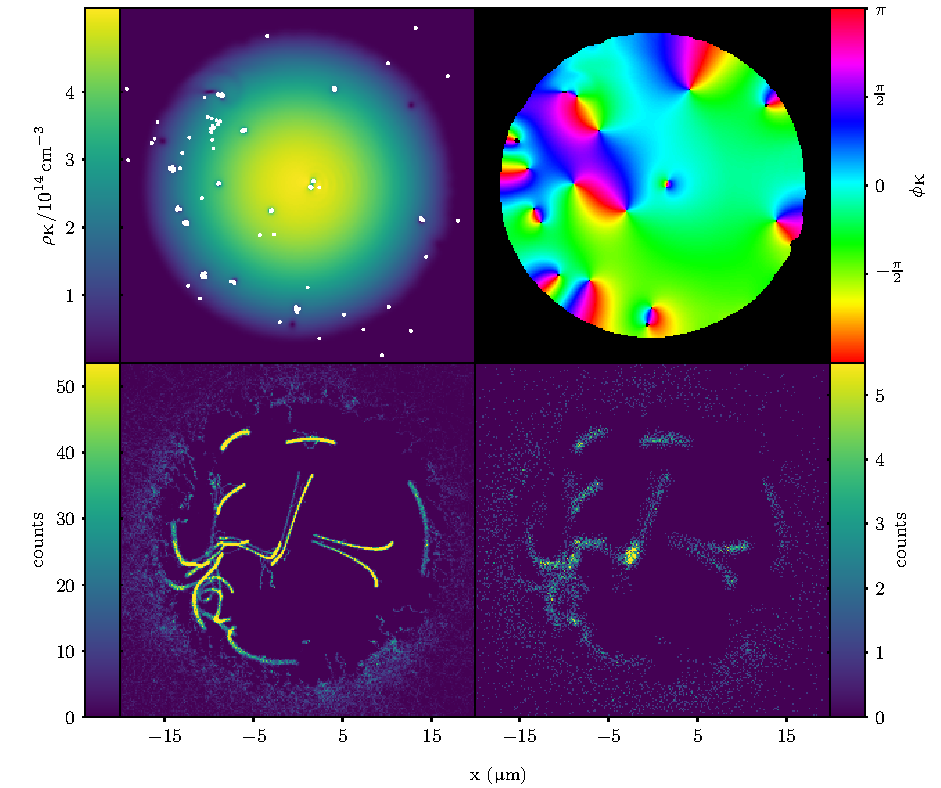
\includegraphics{figures/velocimetry/imaging_high_densitylate_start.pdf}
\caption{Final state of the higher density simulation of imaging of tracer particles in the \textsc{bec} for $10\unit{ms}$ starting from the state of the `dark' simulation at $32\unit{ms}$ (i.e.~the rightmost pair of Figure~\ref{fig:evolution_high_density}). Top left: The condensate density (false colour) and tracer particle positions (white dots). Top right: condensate phase, showing the position of vortices as points about which phase winds by $2\pi$. Bottom left: idealised image of tracer particle photon emissions over the imaging period. Photon emission locations are binned into a $256\times256$ grid. Vortex motion is visible, with slightly better contrast than in Figure~\ref{fig:imaging_high_densitynormal_start}, owing to fewer vortex annihilations taking place in this time interval, though the difference is minor. Bottom right: modelled image taking into account non-unity collection efficiency and diffraction. Photon counts are low, but vortex motion is still visible. Here the increased clarity of the vortex motion over~Figure~\ref{fig:imaging_high_densitynormal_start} is more apparent.}\label{fig:imaging_high_densitylate_start}
\end{figure}
\restoregeometry
}

\afterpage{
    \newgeometry{left=1in,bottom=1in,right=1in,top=1.5in}
    \begin{sidewaysfigure}[th]
    \centerfloat
    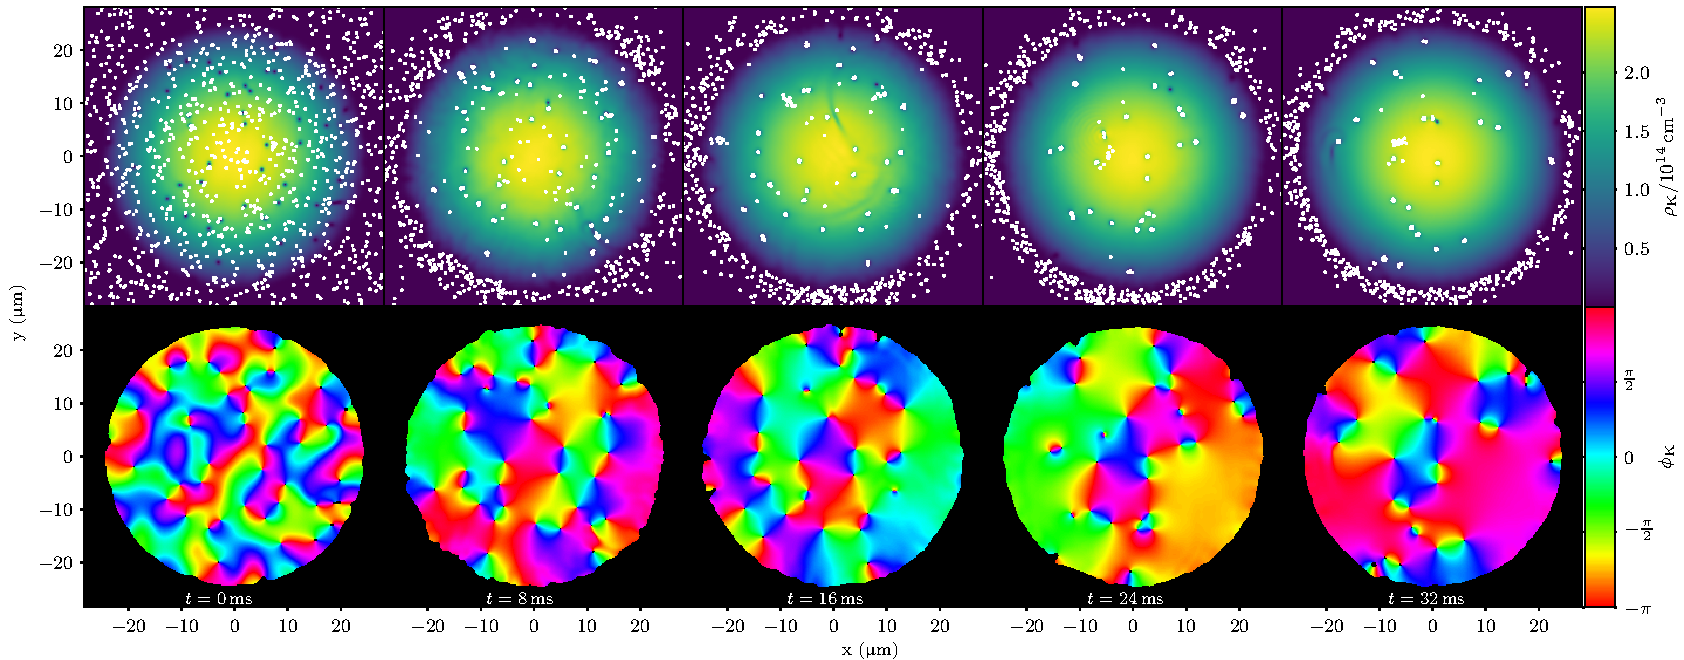
\includegraphics[width=1.05\textwidth]{figures/velocimetry/evolution_low_density.pdf}
    \caption{Lower density simulation of the evolution over time of the potassium condensate and $10^3$ rubidium tracer particles interacting via sympathetic cooling, beginning from a turbulent condensate with randomly distributed tracer particles. Top row: condensate density (false colour) and tracer particle positions (white dots). Bottom row: condensate phase showing the location of vortices as points about which the phase winds by $2\pi$. The initially randomly distributed tracer particles either leave the condensate or become trapped in vortex cores.}
    \label{fig:evolution_low_density}
    \end{sidewaysfigure}
    \restoregeometry
}


\afterpage{
\newgeometry{left=1in,bottom=1.5in,right=1in,top=1.5in}
\begin{figure}
\centerfloat
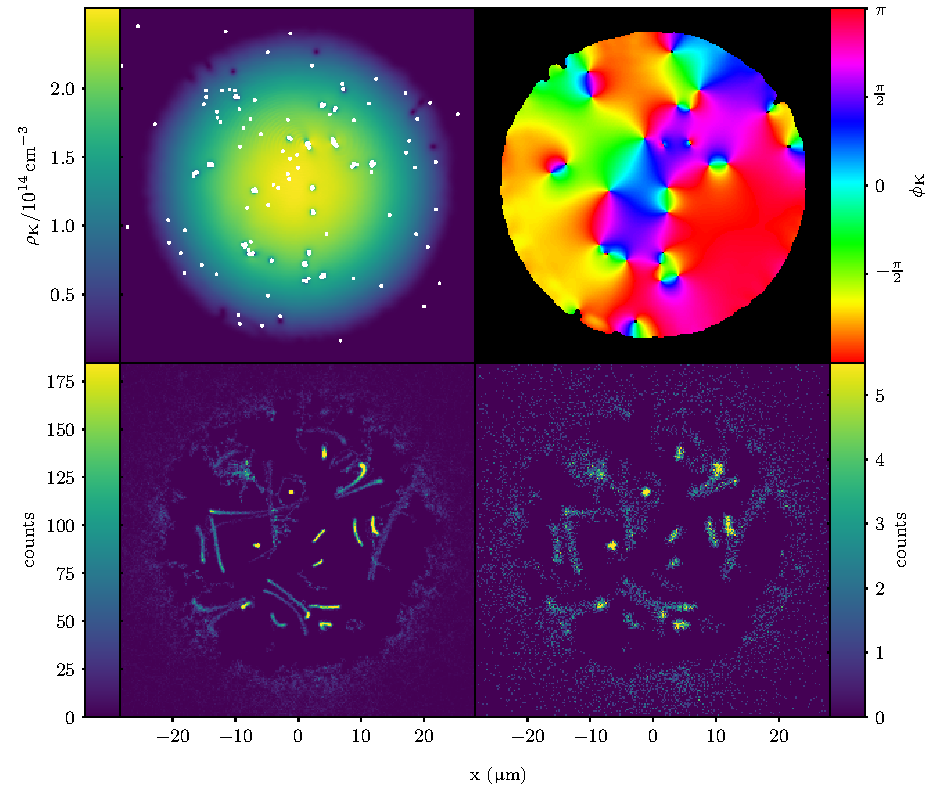
\includegraphics{figures/velocimetry/imaging_low_densitynormal_start.pdf}
\caption{Final state of the lower density simulation of imaging of tracer particles in the \textsc{bec} for $10\unit{ms}$ starting from the state of the `dark' simulation at $16\unit{ms}$ (i.e.~the central pair of Figure~\ref{fig:evolution_low_density}). Top left: The condensate density (false colour) and tracer particle positions (white dots). Top right: condensate phase, showing the position of vortices as points about which phase winds by $2\pi$. Bottom left: idealised image of tracer particle photon emissions over the imaging period. Photon emission locations are binned into a $256\times256$ grid. Vortex tracks appear shorter than in the higher density simulations, owing to the slower vortex velocity at lower density. Tracer particles are clearly still able to remain trapped despite the shallower vortex potentials, and the slower vortex velocity improves contrast as more photons are emitted per unit distance of vortex motion. Bottom right: modelled image taking into account non-unity collection efficiency and diffraction. Photon counts are low, but vortex motion is still visible. The increased clarity of vortex tracks due to their slower motion is still apparent with the lower photon counts. As the lower condensate is larger, diffraction is slightly less apparent than in the higher density simulations.}\label{fig:imaging_low_densitynormal_start}
\end{figure}
\restoregeometry
}

\afterpage{
\newgeometry{left=1in,bottom=1.5in,right=1in,top=1.5in}
\begin{figure}
\centerfloat
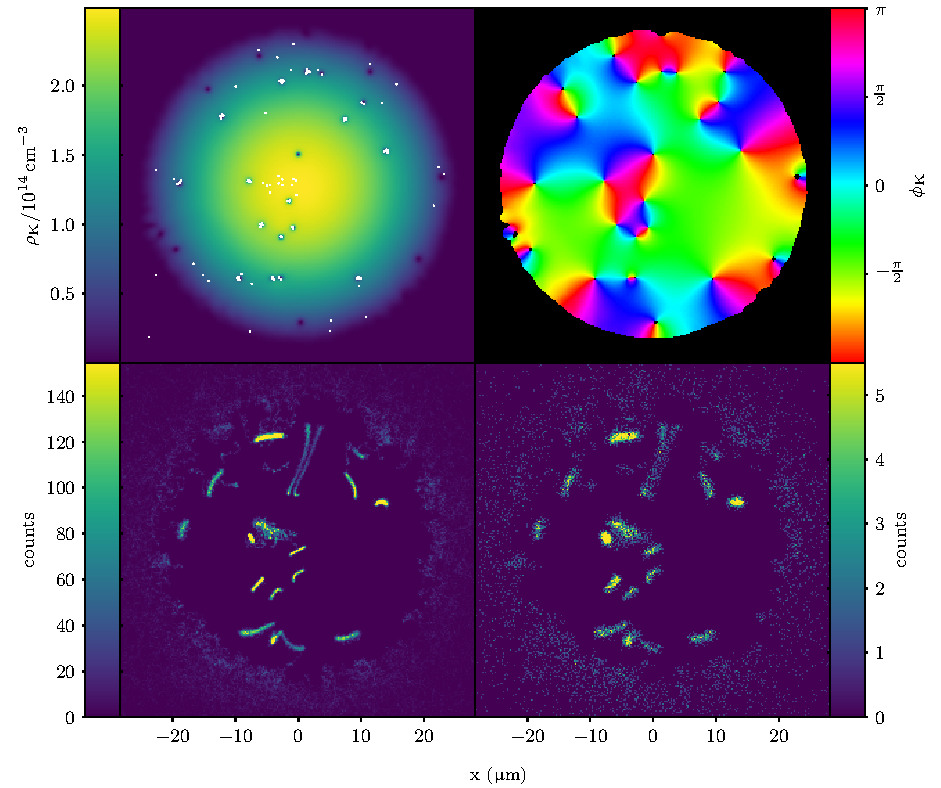
\includegraphics{figures/velocimetry/imaging_low_densitylate_start.pdf}
\caption{Final state of the lower density simulation of imaging of tracer particles in the \textsc{bec} for $10\unit{ms}$ starting from the state of the `dark' simulation at $32\unit{ms}$ (i.e.~the rightmost pair of Figure~\ref{fig:evolution_low_density}). Top left: The condensate density and tracer particle positions (white dots). Top right: condensate phase, showing the position of vortices as points about which phase winds by $2\pi$ (phase only plotted where density is $>5\%$ of maximum density). Bottom left: idealised image of tracer particle photon emissions over the imaging period. Photon emission locations are binned into a $256\times256$ grid. Vortex tracks are shorter than in the higher density simulations due to slower vortex motion, and there are fewer of them owing to more vortex annihilation occurring before the imaging light was turned on. Bottom right: modelled image taking into account non-unity collection efficiency and diffraction. This is perhaps the clearest image of vortex motion out of the four imaging simulations, with vortex trails most clearly visible and separated owing to their lower number and slower velocity.}\label{fig:imaging_low_densitylate_start}
\end{figure}
\restoregeometry
}

\clearpage

\section{Sisyphus cooling in a $34\unit{G}$ magnetic field}\label{sec:laser_cooling_simulations}

As mentioned, one of the limitations of the usual method of polarisation gradient cooling is that it doesn't work in a magnetic field larger than $\Gamma/\gamma$, where $\Gamma$ is the transition line width and $\gamma$ the gyromagnetic ratio. Fields larger than this cause some of the required transitions to shift out of resonance which destroys the cooling effect. Usually this is not an issue for the cooling stage used en-route to \bec; the magnetic field is simply temporarily switched off. Our imaging method would benefit from a cooling scheme that does work in a magnetic field, since the repulsive interactions between $^{87}$Rb and $^{41}$K can be greatly enhanced via a Feshbach resonance at $34 \unit{G}$~\cite{thalhammer_double_2008}. This would make the potential wells that the rubidium atoms see deeper, trapping them more strongly. However if the magnetic field destroys the cooling mechanism then the atoms won't stay trapped for long. Even if sympathetic cooling is sufficient to image tracer particles trapped in vortices, the addition of a cooling scheme would increase the lifetime of the condensate on account of decreased sympathetic heating, and may allow a larger scattering rate of photons before the tracer atoms cease to be trapped.

The Feshbach resonance only occurs if both species are in their respective \mbox{$\ket{S_{1/2}, F=1,m_F=1}$} states,\footnote{$F$ is not a good quantum number in a nonzero magnetic field, so what we mean writing this is the state that one would get if starting in an $F$ state and adiabatically turning on the magnetic field.} so a cooling mechanism in which the rubidium atoms spend a significant fraction of their time in this state is desirable.

In this section I present a sub-Doppler cooling scheme that is designed to cool $^{87}$Rb in a $34\,$G magnetic field. The basic Sisyphus mechanism---of atoms moving alternately between spin states which see different potentials---is possible to find in many multi-level systems of sufficient complexity\footnote{And indeed, many other Sisyphus cooling mechanisms exists other than polarisation gradient cooling~\cite[p 116]{metcalf_laser_1999}.}; my cooling scheme uses a Sisyphus mechanism with four lasers to cool and repump $^{87}$Rb atoms in a $34\unit{G}$ field, with the atoms spending approximately half their time in the \mbox{$\ket{S_{1/2}, 1,1}$} state.

In Section~\ref{sec:vortexcooling}, I briefly describe another cooling scheme suggested by Prof.~Helmerson, which uses the vortex cores themselves as the potential hills in a Sisyphus mechanism. I have not simulated this scheme to asses its viability; I mention it here because it is illustrative of the type of problem that is difficult to model semiclassically, and was one of the factors that led me to consider the use of hidden variables in semiclassical models, as discussed in Chapter~\ref{chap:hvsc}.


\subsection{Description of cooling scheme}

\begin{figure}
\begin{center}
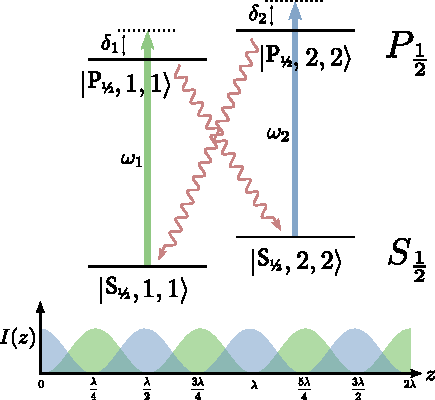
\includegraphics[width=0.65\textwidth]{figures/unsorted/cooling_simplified.pdf}
\caption{\label{fig:cooling_simplified}An idealised depiction of the cooling scheme, with repump lasers and undesired states not shown. Two lasers on the $D_1$ line are used for cooling, both linearly polarised, with the relative phases of all beams fixed so as to form two interleaved standing waves, with the nodes of one standing wave coinciding with the anti-nodes of the other. Both are blue detuned from the transitions they target, and they differ by about $6.8\,$GHz. This difference means that the alignment of the two standing waves can only be maintained over a distance of about a centimetre.}
\end{center}
\end{figure}

The scheme involves four lasers, two for cooling and two for repumping. For simplicity I will first focus on the cooling lasers only, depicted in Figure~\ref{fig:cooling_simplified}. Consider a rubidium atom at $z=0$ and in the $\ket{S_{1/2}, 1,1}$ hyperfine ground state. At this position the atom sees no light, as the intensity of the cooling laser labelled $\omega_1$ is zero, and it is in the wrong state to be pumped by the $\omega_2$ laser (which is not resonant with any transitions from the $\ket{S_{1/2}, 1,1}$ ground state).

As the atom moves rightward however, it will have to climb the repulsive potential hill formed by the $\omega_1$ laser. As it does so, its $\ket{P_{1/2}, 1,1}$ excited state probability will increase, and along with it, the probability of spontaneous emission. Spontaneous emission will be most likely to occur near the top of the potential hill where the laser intensity---and hence the excited state probability---is greatest.

The most likely ground state for the atoms to decay to from the $\ket{P_{1/2},1,1}$ excited state is the $\ket{S_{1/2}, 2,2}$ ground state, and this is most likely to occur near $z=\frac\lambda4$. If this occurs, we now have an atom in the $\ket{S_{1/2},2,2}$ ground state at $z=\frac\lambda4$, a situation similar to that in which it started. Again, out atom now sees no light, but which laser has zero intensity and which targets the wrong transition are swapped.

As our atom continues rightward, it now has to contend with the potential hill formed by the $\omega_2$ laser, and is most likely to undergo spontaneous emission from the $\ket{P_{1/2},2,2}$ excited state near the top of the potential hill. This time emission is most likely to put the atom into the $\ket{S_{1/2},1,1}$ ground state.

This process repeats, with atoms repeatedly climbing potential hills and being cooled. They spend approximately half their time in the $\ket{S_{1/2},1,1}$ ground state, allowing us to take advantage of the strong interspecies repulsion that that state entails for our two atomic species.

Of course, as is always the case, things aren't that simple. Whilst the two spontaneous decays mentioned above are the most likely, they are by no means the only possibilities. Some spontaneous decays will put the atoms back into the ground state from which they came, with no harm done except a little extra heating from the photon recoil. Other decays however will put our atom into states that are not involved in the cooling scheme, where they will remain with no further cooling unless we do something about it. For this we need repump lasers (Figure~\ref{fig:cooling_full}).

There are three states that the atom might end up in as a result of decay from the two excited states involved in the cooling process, and two repump lasers are used to excite them to three $P_{3/2}$ states,\footnote{I chose the $P_{3/2}$ manifold as the target of the repump transitions so that they would not interfere with the cooling cycle---repump beams that addressed the same $P_{1/2}$ states as the cooling beams would cause coherent population transfer into the undesired states.} from where they can spontaneously decay back to states in the cooling cycle. Two of these transitions are similar enough that they can be addressed with the same laser.

\begin{figure}
\begin{center}
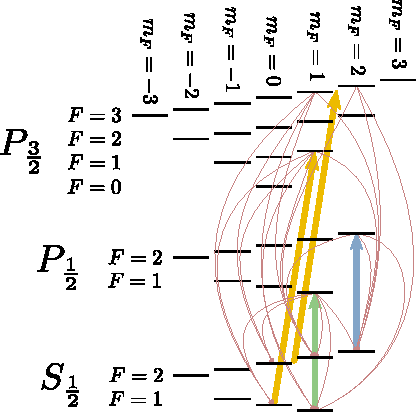
\includegraphics[width=0.65\textwidth]{figures/unsorted/cooling_full.pdf}
\caption{The full cooling scheme, including repump lasers (yellow), cooling lasers (blue and green), and all possible decay paths (red). The repump beam which is drawn in between two ground and excited states has a frequency equal to the average of those two transitions.}\label{fig:cooling_full}
\end{center}
\end{figure}

\subsection{Methods}

The cooling scheme was simulated for the case of a single atom, with the internal state of the atom modelled with the Schr\"odinger equation in the eigenbasis of the hyperfine and Zeeman Hamiltonians (described in Section~\ref{sec:the_rubidium_D_line}), comprising $32$ states. The dipole transition matrix elements coupling each pair of states were each computed as the appropriate linear sum of the dipole matrix elements at zero field, using the dipole approximation and the rotating wave approximation, as described in Section~\ref{sec:optical_dipole_transitions}. Since the corresponding Rabi frequencies depend on the laser intensity as well as the dipole matrix elements, they are functions of space, to be computed at each integration timestep as the atom moves through different intensities of the cooling beams. Following~\cite[p 4]{metcalf_laser_1999}, this produced a set of 32 coupled differential equations for the amplitudes of each state, of the form :

\begin{equation}
\ii\hbar\dv{t} c_e(t) = -\frac12e\sum_{g,\ n} E_n \langle g |  q_n | e \rangle c_g(t) \ee^{-\ii\delta_{nge}t},
\end{equation}
and
\begin{equation}
\ii\hbar\dv{t} c_g(t) = -\frac12e\sum_{e,\ n} E_n \langle g |  q_n | e \rangle c_e(t) \ee^{\ii\delta_{nge}t},
\end{equation}
where each $c(t)$ is the complex amplitude of one state; the $e$ indices are over the excited states and the $g$ indices over the ground states; the $n$ indices are over the lasers, with $E_n$ being the $n$\textsuperscript{th} laser's electric field, $\delta_{nge}$ the detuning of the $n$\textsuperscript{th} laser from the $g\rightarrow e$ transition, and $\matrixel{g}{q_n}{e}$ the dipole moment between the $g$\textsuperscript{th} ground and $e$\textsuperscript{th} excited states for the polarisation $q_n$ of the $n$\textsuperscript{th} laser.

The external motion of the atom was modelled classically, with the atom having a definite position and velocity in one dimension. The force on the atom was computed from the dipole forces that the two ground states involved in the cooling cycle experience due to the standing waves formed by the cooling beams. An expectation value of the dipole force was computed as:
\begin{align}
\ev{F} = \abs{\braket{S_{1/2},1, 1}{\Psi}}^2F_{\ket{S_{1/2},1, 1}} + \abs{\braket{S_{1/2}, 2, 2}{\Psi}}^2F_{\ket{S_{1/2},2, 2}},
\end{align}
where $F_{\ket{S_{1/2}, 1, 1}}$ and $F_{\ket{S_{1/2}, 2, 2}}$ are the dipole forces on the two ground states, calculated using~\cite[eqn 3.16, p 33]{metcalf_laser_1999} with one standing wave offset from the other by a quarter wavelength. The forces on other ground states are neglected since the repump beams do not have intensity gradients, and since the cooling beams are much further away from resonance for ground states other than the two in the cooling cycle. Forces on excited states are also neglected. The forces on the two excited states in the cooling cycle are not smaller than those on the corresponding ground states, however the excited state populations are small since the cooling beams are several line widths away from resonance.

This expectation value of the dipole force was used to model the classical motion of the atom. Although the components of an atom in superposition would in reality spatially separate under the influence of a force that is different for different internal states of the atom, as in the Stern--Gerlach experiment, our atom only transitions between the two states subject to different forces via spontaneous emission, after which it is in an eigenstate. Accordingly, the expectation value calculation is always dominated by one of the two ground states and the potential for Stern--Gerlach separation does not arise.

Spontaneous emission was simulated stochastically at each integration timestep, with probability of decay per unit time equal to the sum of populations in all excited states, multiplied by their decay rates (equal to the natural line widths of each of the two fine-structure lines). Multiplying by the duration of one timestep, and comparing with a random number then determined whether a decay was to occur.

In the event of a decay, one excited state was randomly chosen with probability proportional to its population, and then one ground state, weighted by the transition strengths from the excited state. All population was then put into that ground state and the simulation continued, with one photon of momentum in a random \textsc{1d} direction added to the atom's momentum to account for photon recoil.

The equations of motion were solved using fourth order Runge--Kutta integration (Section~\ref{sec:rk4})

\subsection{Results}

\begin{table}
    \renewcommand{\arraystretch}{2.0}
    \makebox[\textwidth][c]{
    \begin{tabular}{|c|p{3.5cm}|r|r|c|}\hline
    Type & Transition(s) & Detuning & \shortstack{\\Intensity\\(per beam)} & Polarisation\\\hline
    \shortstack{\\cooling\\(standing wave)} & $|S_{1/2},2,2\rangle\rightarrow |P_{1/2},2,2\rangle$ & + $66.6\,$MHz & $5.0\,$mW$\,$cm$^{-2}$ & $\pi$ \\\hline
    \shortstack{\\cooling\\(standing wave)} & $|S_{1/2},1,1\rangle\rightarrow |P_{1/2},1,1\rangle$ & + $31.9\,$MHz & $5.0\,$mW$\,$cm$^{-2}$ & $\pi$ \\\hline
    \shortstack{\\repump\\(single beam)} & \shortstack{\\ $|S_{1/2},2,1\rangle\rightarrow |P_\frac32,2,2\rangle$ \\
                           $|S_{1/2},2,0\rangle\rightarrow |P_\frac32,2,1\rangle$} & \shortstack{\\\\Midway\\between} & $50.0\,$mW$\,$cm$^{-2}$ & $\sigma^+$ \\\hline
    \shortstack{\\repump\\(single beam)} & $|S_{1/2},1,0\rangle\rightarrow |P_\frac32,1,1\rangle$  & $0$ & $10.0\,$mW$\,$cm$^{-2}$ & $\sigma^+$ \\

    \hline
    \end{tabular}
    }
    \caption{The parameters used in the laser cooling simulations. There are four lasers, each with a specified polarisation, intensity, and detuning from the transition it targets.}\label{table:numbers}
\end{table}

The laser parameters used in the simulation are shown in Table~\ref{table:numbers}. The magnetic field strength used was $34\unit{G}$. The detunings of the cooling beams were chosen based on an approximate calculation in order to produce a scattering rate of $2\times10^{5}$ photons per second in the simulation.

The simulation was run for $7.2\times10^6$ integration timesteps of size $\upDelta t=20\unit{ps}$,\footnote{Corresponding to approximately ten timesteps per oscillation of the fastest oscillating terms, which oscillate at a rate close to half the $6.8\unit{GHz}$ hyperfine splitting of the rubidium ground states.} for a total of 14.3 milliseconds of simulation time. This took $14$ days of computer time. In that time, the atom moved a maximum distance of $26\unit{\upmu m}$ from its starting position, and its final position was $790\unit{nm}$ from its starting position. The atom's initial velocity was $195 \unit{mm\,s}^{-1}$, and during the simulation it reversed the direction of its velocity $2226$ times; $4103$ photons were emitted, for an average scattering rate of $2.87\times10^\up{5}$ photons per second---slightly higher than the target rate.

I computed the time-averaged kinetic energy of the atom over the whole simulation as:
\begin{equation}
\ev{E_\up{K}} = \frac12 m_\up{Rb} \langle v^2 \rangle.
\end{equation}
Assuming the single atom ergodically sampled a sufficient fraction of the possible state space, one can compute from this the \textsc{1d} temperature that a cloud of atoms subject to this cooling would have, after being allowed to come to equilibrium using
\begin{align}
\frac12 k_\up{B} T_\up{1D} = \ev{E_\up{K}}.
\end{align}
This gave $T_\up{1D} = 16.2\unit{\upmu K}$, well below the Doppler temperature $T_\up{D} = 146\unit{\upmu K}$~\cite{steck_rubidium_2015}. A histogram showing the time the atoms spent at different velocities is shown in Figure~\ref{fig:cold_atom}. This one-dimensional temperature corresponds to $\approx30E_\up{r}$ where $E_\up{r}$ is the rubidium recoil energy. Given that the potassium vortex potentials are at about $15E_\up{r}$ deep without a Feshbach resonance at a density of $1\times10^{15}\unit{cm}^{-3}$ and only $\approx 2.0E_\up{r}$ at the more realistic density of $1\times10^{14}\unit{cm}^{-3}$, and that the atom only spends about half its time in the state subject to the Feshbach resonance, this cooling would only be sufficient to keep rubidium atoms trapped in vortex cores if the Feshbach resonance enhances the interspecies scattering length by a factor of $\approx 2$ for a $1\times10^{15}\unit{cm}^{-3}$ condensate or a factor of $\approx 30$ for a $1\times10^{14}\unit{cm}^{-3}$ condensate. While a factor of $2$ is easily achievable, a factor of $30$ is not, indicating that the minimum density compatible with tracer particles at this temperature being trapped is between $1\times10^{14}\unit{cm}^{-3}$ and $1\times10^{15}\unit{cm}^{-3}$.

\begin{figure}
\begin{center}
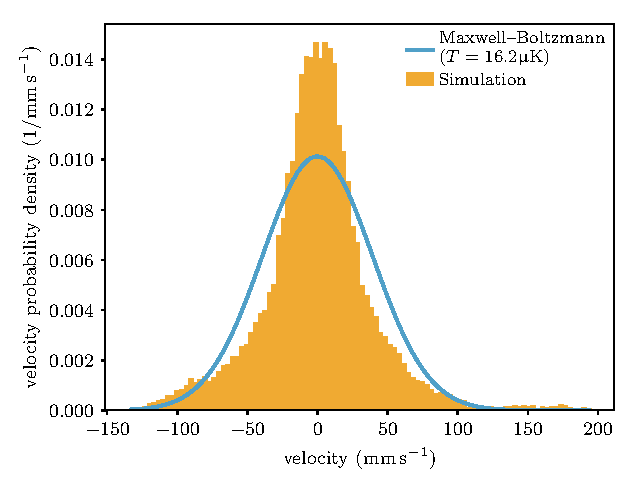
\includegraphics[width=\textwidth]{figures/velocimetry/laser_cooling_results.pdf}
\caption{\label{fig:cold_atom} Histogram in orange of atom velocity, normalised as a probability density. The symmetry about zero velocity and low level of noise on the histogram is good evidence that the atom ergodically sampled the range of possible velocities such that the histogram can be interpreted as a probability distribution. The long tail visible to the right is the atom's initial slowdown from its starting velocity. A Maxwell--Boltzmann distribution with the same mean kinetic energy is shown as the blue line. It is no surprise that it does not agree with the histogram---there is no thermalisation happening since there is only one atom and no collisions---but this represents the distribution that a cloud of atoms with the same per-particle mean kinetic energy as our atom would thermalise to in the presence of collisions.}
\end{center}
\end{figure}

This simulation has not, however, been optimised---the results presented here represent the only extended simulation of the scheme, and no attempt has been made to scan over parameter space to see if the temperature can be made lower. As mentioned the simulation was computationally expensive, and so optimisation would be impractical if performed using the same code. However, a significant speed up would be possible by correcting some inefficiencies. Firstly, one could exclude from the simulation the atomic states that were shown in the first run never to become occupied---the states with no arrows leading to them in \figref{fig:cooling_full}. This will eliminate approximately two thirds of the states, and since the simulation is quadratic in the number of states, this should provide an approximately $10\times$ increase in simulation speed. More importantly, lasers that are detuned with respect to a given transition by approximately the hyperfine splitting of $6.8\unit{GHz}$ should be discarded in the coupling term for that transition. The inclusion of these fast rotating terms---which are so far detuned as to cause negligible population transfer---was the limiting factor in the simulation timestep size, which would otherwise be determined by the next fastest rotating terms on the order of tens of $\unit{MHz}$ instead of $\unit{GHz}$. This would lead to a likely dramatic speedup as well, making repeated runs of the simulation feasible.

\subsection{Vortex-assisted Sisyphus cooling}\label{sec:vortexcooling}

Another idea for a cooling scheme is to use the vortex potential itself as a spatial discriminator for transferring atoms between states. Similar to how a \mot\ traps atoms by bringing them into resonance with optical pumping only when they are some distance from the trap centre, one might use the shape of the vortex potential to bring an \rf\ or microwave transition into resonance only when trapped tracer particles are some distance away from the centre of a vortex core. This method was proposed by Prof.~Helmerson whilst considering different possibilities for cooling atoms in vortex cores, and I considered which states might be appropriate to implement the scheme in. I have not simulated this scheme, but present it here because the reason it is difficult to simulate is an example of the type of problem that led me to develop the hidden variable semiclassical method presented in Chapter~\ref{chap:hvsc}.

\begin{figure}
\begin{center}
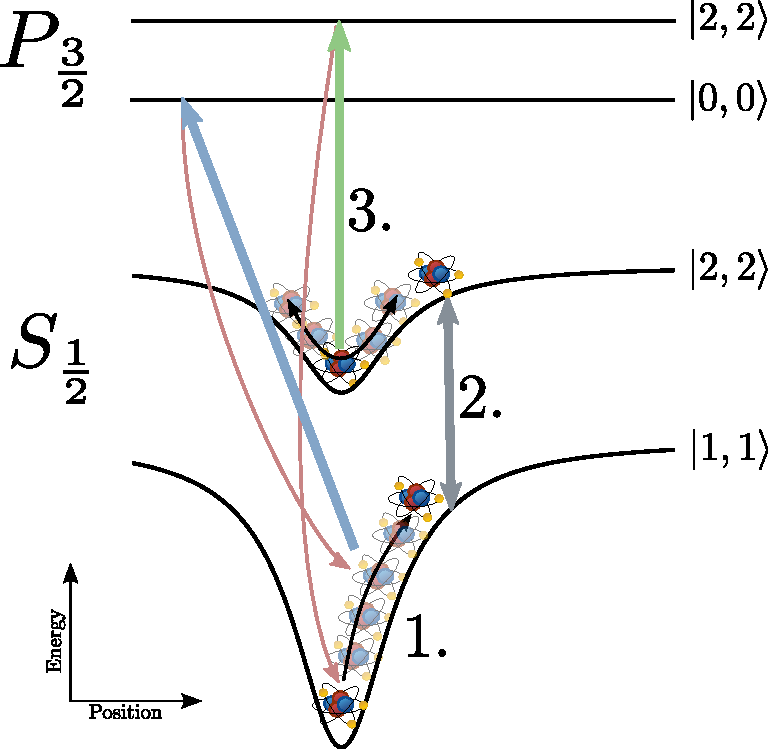
\includegraphics[width=0.7\textwidth]{figures/unsorted/vortexcooling.pdf}
\caption{A basic description of the vortex-assisted cooling scheme. 1. The rubidium atom in its $\ket{S_{1/2}, 1,1}$ ground state repeatedly scatters photons from the laser marked with the blue arrow, climbing the vortex potential as it does so. The optical transition's line width is large enough that the energy shift due to the vortex potential does not move it off resonance (and this allows us to ignore the vortex potentials experienced by the excited state, not shown). 2. An \rf\ or microwave transition however, has an extremely narrow line width; its effective line width is dependent only on the \rf/microwave power. A microwave transition (grey arrow) comes into resonance only when the atom moves sufficiently far from the vortex core's centre, and coherently transfers population into the $\ket{S_{1/2}, 2,2}$ ground state. 3. The atom oscillates back and forth in the much shallower vortex potential that its $\ket{S_{1/2}, 2,2}$ ground state experiences. It is pumped weakly by the laser marked with the green arrow, and after a random time delay (and hence at a random position) spontaneously decays back to the $\ket{S_{1/2}, 1,1}$ ground state.
}\label{fig:vortexcooling}
\end{center}
\end{figure}

The basic idea of the vortex-assisted cooling scheme is outlined in Figure~\ref{fig:vortexcooling}. In the presence of the Feshbach resonance, atoms in the $\ket{S_{1/2}, 1,1}$ state scatter some tens of photons, using whichever transition is most likely to have them decay to the same ground state with minimal repumping (the $\ket{P_{3/2}, 0,0}$ excited state on the $D_2$ line looks to be the best choice). As the atom scatters photons, it climbs the side of the vortex potential, converting the kinetic energy obtained from photon recoil into potential energy.

Due to the state-dependence of the interspecies scattering length, the vortex potentials for different states have different depths, especially when one is enhanced by a Feshbach resonance. This means that the \rf\ or microwave frequency required to transition between the different hyperfine states and Zeeman sublevels varies as a function of space, and can be tuned so as to only be resonant with atoms which have nearly escaped the vortex core.

When the atom enters the region resonant with said \rf\ or microwave radiation, it is then transferred into a different hyperfine or Zeeman state, for example the $\ket{S_{1/2}, 2,2}$ ground state, and the hope is that it then lacks the kinetic energy to escape the (shallower) vortex potential it then finds itself in. Rather, it oscillates back and forth in the well until a weak laser pumps it back into the $\ket{S_{1/2}, 1,1}$ ground state via spontaneous emission from some excited state (again chosen to maximise the decay probability to $\ket{S_{1/2}, 1,1}$; the $\ket{P_{3/2}, 2,2}$ excited state looks to be a good choice.)

After completing this cycle, statistically the atom will be closer to the centre of the  $\ket{S_{1/2}, 1,1}$ vortex potential than when it left the $\ket{S_{1/2}, 1,1}$ state. Provided the corresponding drop in potential energy makes up for the photon scattering (which provides fluorescence imaging), then it comprises a cooling and imaging scheme capable of keeping the atoms trapped in the vortex cores. It is yet another Sisyphus effect, with the atom climbing steep vortex potential hills and descending shallower ones.

However, this scheme cannot be simulated in the same manner as the laser cooling scheme presented in Section~\ref{sec:laser_cooling_simulations}. The reason is that the \rf\ or microwave transition depicted as the grey arrow in~\figref{fig:vortexcooling} is coherent, and as such leads to state vectors that are superpositions of the two hyperfine or Zeeman sublevels, with no one state dominating the superposition.\footnote{This is in contrast to the cooling scheme presented in Section~\ref{laser_cooling_simulations}, in which population was primarily on one of two ground states, and switched between them only via spontaneous emission} Since (crucially for the cooling scheme), the two states are subject to different potentials, an atom in such a superposition would undergo Stern--Gerlach separation. Unlike the laser cooling scheme from the previous section, since no one state dominates the superposition at a given time, the expectation value of the two forces does not accurately describe the motion of the atom. To accurately simulate this cooling scheme, a semiclassical method able to reproduce this Stern--Gerlach separation would likely be necessary. This realisation, along with similar difficulties in simulations of Majorana losses in evaporative cooling during collaboration with Drs.~Turner and Anderson and Chris Watkins led me to develop the hidden-variable semiclassical method, discussed in Chapter~\ref{chap:hvsc}.

\section{Conclusion}

The sympathetic cooling results shown in Section~\ref{sec:sympathetic} are promising, indicating that it is likely possible to observe vortex motion in \textsc{bec}s of realistic density via tracer particles using a Feshbach resonance and no additional cooling. A limitation of these results is their neglect of the corresponding sympathetic heating of the condensate, which could limit the duration over which vortices can be imaged. Furthermore, the assumption of solely elastic collisions becomes increasingly inaccurate as larger Feshbach-induced scattering enhancements are used due to an enhancement of inelastic collisions~\cite{stenger_strongly_1999}. A final limitation is that in three dimensions, the halo of atoms that have left the condensate but are still trapped would also be in front of the condensate from the perspective of the imaging system, which would obscure the view of the tracer particles within the condensate somewhat.

The new laser cooling method presented in Section~\ref{sec:laser_cooling_simulations} appears---in simulation--to be able to provide sub-Doppler cooling at the magnetic field strength required for the $^{41}$K--$^{87}$Rb Feshbach resonance. It is however an admittedly cumbersome method from an experimental perspective. It requires four lasers, driving transitions on both $D$ lines from both hyperfine ground states. It requires relative phase control over the two cooling beams such that their standing waves are correctly aligned with the intensity troughs of one at the peaks of the other. These two beams are detuned from each other by the $6.8\unit{GHz}$ hyperfine splitting of the ground state, and so their wavelengths are different enough that this alignment can only be maintained over a distance on the order of $1\unit{cm}$. Although the simulation was only in one spatial dimension, a similar arrangement of interlocking standing waves is possible in \textsc{2d} to provide cooling in the two directions orthogonal to the magnetic field. However, since it is not possible for a beam with propagation direction parallel to the magnetic field to provide $\pi-$polarised light, one could not use the scheme in \textsc{3d} for cooling in all three directions. Finally, although the cooling scheme did not appear to provide sufficient cooling for trapping in vortex cores, as mentioned it has not been optimised, and so may be capable of cooling to lower temperatures.